% This is samplepaper.tex, a sample chapter demonstrating the
% LLNCS macro package for Springer Computer Science proceedings;
% Version 2.20 of 2017/10/04
%
\documentclass[runningheads]{llncs}
%
\usepackage{graphicx}
\usepackage{color}
\usepackage{amsmath}
\usepackage{amsfonts}
\usepackage{amssymb}
\usepackage{multirow}
\usepackage{multicol}
\usepackage{tabularx}
\usepackage{tikz}
\usepackage{pgfplots}
\usepackage{pgfplotstable}
\usepackage{lmodern}
\usepackage{pgffor}

% Used for displaying a sample figure. If possible, figure files should
% be included in EPS format.
%
% If you use the hyperref package, please uncomment the following line
% to display URLs in blue roman font according to Springer's eBook style:
% \renewcommand\UrlFont{\color{blue}\rmfamily}
\usetikzlibrary{matrix}
\usepgfplotslibrary{groupplots}
\pgfplotsset{compat=newest}

\setlength{\parindent}{0pt}
\renewcommand{\indent}{\hspace*{0pt}}

\newcommand{\tab}{\hspace*{3mm}}
\newcommand{\tabs}[1]{\foreach \n in {1,...,#1}{\tab}}
\newcommand{\qtab}{\hspace*{3mm} \ \quad}
\newcommand{\qtabs}[1]{\foreach \n in {1,...,#1}{\qtab}}

\newcommand{\sif}[3]{\text{if } #1 \text{ then } #2 \text{ else } #3}
\newcommand{\product}[2]{#1 \times #2}
\newcommand{\tuple}[2]{(#1 :: #2)}
\newcommand{\rearrs}[3]{RearrS \ #1 \ #2 \ #3}
\newcommand{\rearrv}[3]{RearrV \ #1 \ #2 \ #3}
\newcommand{\casebx}[4]{Case \ #1 \ #2 \ #3 \ #4}

\newcommand{\putbx}[3]{put \, [\![#1]\!] \ #2 \ #3}
\newcommand{\putbxinline}[1]{put \, [\![#1]\!]}
\newcommand{\getbx}[2]{get \, [\![#1]\!] \ #2}
\newcommand{\getbxinline}[1]{get \, [\![#1]\!]}

\newcommand{\putrev}[3]{put_{REV} \, [\![#1]\!] \ {#2} \ {#3}}
\newcommand{\getrev}[2]{get_{REV} \, [\![#1]\!] \ {#2}}

\newcommand{\pg}[3]{pg \, [\![#1]\!] (#2, #3)}
\newcommand{\pginline}[1]{pg \, [\![#1]\!]}

\newcommand{\cpg}[5]{cpg [\![#1]\!] (#2, #3, #4, #5)}
\newcommand{\cpginline}[1]{cpg \, [\![#1]\!]}

\newcommand{\kpg}[7]{kpg [\![#1]\!] (#2, #3, #4, #5, #6, #7)}
\newcommand{\kpginline}[1]{kpg \, [\![#1]\!]}

\newcommand{\xpg}[3]{xpg \, [\![#1]\!] (#2, #3)}
\newcommand{\xpginline}[1]{xpg \, [\![#1]\!]}

\newcolumntype{L}[1]{>{\raggedright\arraybackslash}p{#1}}
\newcolumntype{C}[1]{>{\centering\arraybackslash}p{#1}}
\newcolumntype{R}[1]{>{\raggedleft\arraybackslash}p{#1}}

\begin{document}
%
\title{An efficient composition of bidirectional programs
  by tupling and lazy updates 
%  tupling
%  accumulating updates = lazy updates
%  based on the idea of reversible computing  
  % \thanks{Supported by organization x.}
}
%
%\titlerunning{Abbreviated paper title}
% If the paper title is too long for the running head, you can set
% an abbreviated paper title here
%
\author{First Author\inst{1}\orcidID{0000-1111-2222-3333} \and
Second Author\inst{2,3}\orcidID{1111-2222-3333-4444} \and
Third Author\inst{3}\orcidID{2222--3333-4444-5555}}
%
\authorrunning{F. Author et al.}
% First names are abbreviated in the running head.
% If there are more than two authors, 'et al.' is used.
%
\institute{Princeton University, Princeton NJ 08544, USA \and
Springer Heidelberg, Tiergartenstr. 17, 69121 Heidelberg, Germany
\email{lncs@springer.com}\\
\url{http://www.springer.com/gp/computer-science/lncs} \and
ABC Institute, Rupert-Karls-University Heidelberg, Heidelberg, Germany\\
\email{\{abc,lncs\}@uni-heidelberg.de}}
%
\maketitle              % typeset the header of the contribution
%
\begin{abstract}
%The abstract should briefly summarize the contents of the paper in
%15--250 words.
  Bidirectional transformation (BX) is a solution of view update problems and widely used for synchronizing data. Its semantics and correctness are researched well, but the efficiency and optimization are not considered well. In this work we focus on the evaluation of composition, because it includes some problems of evaluation time efficiency and memory allocation. To solve these problems we make $put$ and $get$ more tight, based on the idea of tupling. %42
  Because simple tupled result includes some redundancies for left associative compositions, we apply two optimization techniques: lazy update and lazy evaluation. We show some experimental results that our optimized approach is faster than the original approach that is used in an actual BX language.

  
\keywords{Bidirectional transformation  \and Tupling \and Optimization \and ??.}
\end{abstract}
%
%
%

% plan to pages
% abstraction & title & Introduction: 3pages
% miniBiGUL: 1.5page
% pg: 3pages
% cpg: 2page
% kpg: 1page
% xpg:0.5page
% evaluation:2pages
% related work:1page
% conclusion:1page (including reference)
% page limit : 15

%Schedule
\begin{itemize}
%\item Introduction (story), Contribution, positions, examples, beginning of September?
%\item zero draft : mid of September  
%\item deadline of PEPM2020 (October 18th)
%\item ESOP (October 24th)
\item FLOPS 2020, 15 November 2019 (AoE): Abstract submission
\item 22 November 2019 (AoE): Submission deadline
\item keywords, ORCID id, introduction, contribution, future work, related work 
\end{itemize}

%\begin{itemize}
%\item BiGUL 
%\item pg (pair of put and get)
%\item cpg (extention of pg. Keep eval information for reusing)
%\item kpg (extention of cpg. Lazy evaluation)
%\item xpg (combination of pg and kpg)
%\item Experiment
%\item Related work
%\item Conclusion and Future work
%\end{itemize}

\section{Introduction} \label{sec:intro}

%\begin{itemize}
%\item Importance of BX, BX is a solution of view update problem in database.
%\item goodness of
%\item Explanation of put-based BX: BiGUL.
%\item Current status of BiGUL: Fastest BX language in the world
%\item But there is a problem: Efficiency of compose evaluation. The current implementation of BiGUL does not save the intermediate states, the number of get is quadratic. This is not good.
%\item To solve this problem we use an idea: introduce pg : combination of put and get. Then, no information will be lost in a specific condition.
%  an idea from reversible computation: not to lose any information.
%\item We extend pg with several ideas to produce faster implementation.
%\item
%\end{itemize}

%\begin{itemize}
%\item Importance of BX, BX is a solution of view update problem in database.
%\item goodness of
%\item Explanation of put-based BX: BiGUL.
%\item Current status of BiGUL: Fastest BX language in the world
%\item But there is a problem: Efficiency of compose evaluation. The current implementation of BiGUL does not save the intermediate states, the number of get is quadratic. This is not good.
%\item To solve this problem we use an idea: introduce pg : combination of put and get. Then, no information will be lost in a specific condition.
%  an idea from reversible computation: not to lose any information.
%\item We extend pg with several ideas to produce faster implementation.
%\item
%\end{itemize}

%In software, there are strong demands for synchronizing data. In database community this is known as ``the view update problem'' and researched for a long time.
% A Survey to View Update Problem
%As a solution for this problem, bidirectional transformation (BX) is introduced.
The synchronization of data is a common problem. In the database community this problem is known as ``the view update problem'' and has been investigated for a long time~\cite{Bancilhon:1981:USR:319628.319634}. Bidirectional transformation (BX) provides a systematic approach to solving this problem.
Consider a small BX program of $phead$\footnote{The actual program is shown in the next section.}, which consists of two functions: $get$ (for getting the head of an input list) and $put$ (for reflecting the output to the head of the input). Figure \ref{fig:eval-phead} shows an example of the bidirectional behavior of $phead$.
Let $[1,2]$ be the original source~$s$.
The function $get$ is a projection: $get$ of $phead$ picks the first element of the given original source $[1,2]$ and returns $1$ as a view $v$.
%\texttt{get pHead [1,2] = 1}.
%After the view \texttt{v} is obtained, the user can modify the view.
%In this case, the user
%modified the view
%from $1$ to $100$.
%From this updated view, how can the source be updated?
%This is ``the view update problem.''
%To solve this problem, BX provides $put$, an update function on the original source.
%In this example,
Supposing that the view is updated to $100$,
$put$ of $phead$ will construct a new source $s'$ of ${[100,2]}$ from the updated view $v'$ of $100$ and the original source $s$ of $[1,2]$.
%Note that the update to \texttt{s'} uses \texttt{s} and \texttt{v'} as input.
%\texttt{put pHead [1,2] 8 = [8,2]}

\begin{figure}[!t]
  \begin{minipage}{0.3\textwidth}
    \centering
    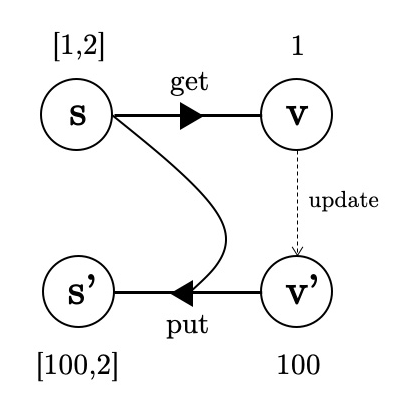
\includegraphics[height=3.5cm]{./fig/fig1.eps}
    \caption{Evaluating $phead$}
    \label{fig:eval-phead}
  \end{minipage}\hfill
  \begin{minipage}{0.7\textwidth}
    \centering
    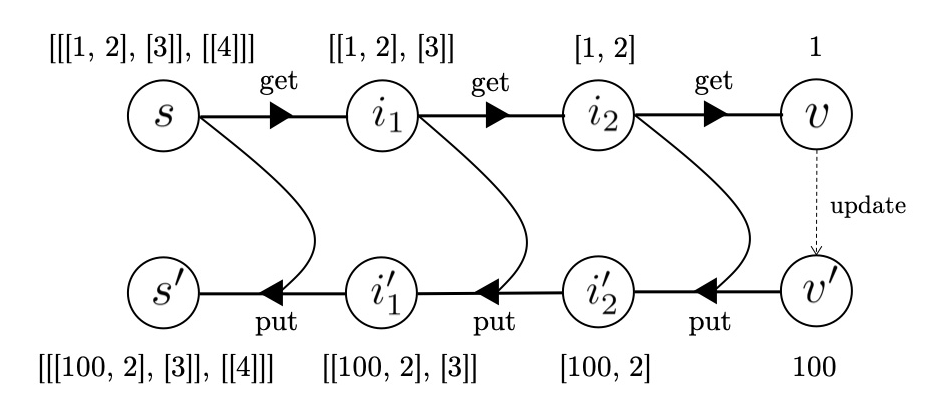
\includegraphics[height=3.5cm]{./fig/fig2.eps}
    \caption{Evaluating $phead~\tilde{\circ}~phead~\tilde{\circ}~phead$}
    \label{fig:eval-comp-phead}
  \end{minipage}
\end{figure}
%\vspace*{-5.5mm}


The composition of BX programs is a fundamental construct to build more complex BX programs \cite{Bohannon06relationallenses:, Bohannon:2008:BRL:1328438.1328487}. Let $bx_1$ (defined by $get_{bx_1}$ and $put_{bx_1}$) and $bx_2$ (defined by $get_{bx_2}$ and $put_{bx_2}$) be two bidirectional programs, then their composition $bx_1 \,\tilde{\circ}\, bx_2$ is defined by

\minusvspace
\begin{align}
get_{bx_1 \tilde{\circ} bx_2}~s &= get_{bx_2} (get_{bx_1}~s)\\
put_{bx_1 \tilde{\circ} bx_2}~s~v' &= put_{bx_1} s~(put_{bx_2}~ (get_{bx_1}~s)~v')
\end{align}
\minusvspace

\noindent
\textcolor{red}{Unlike function composition, the composition of bidirectional programs is read left-to-right. We use this order because it is helpful to understand the behavior if we consider data goes from left to right.}
%\textcolor{red}{Note that the order of composition is the reverse order compared to function composition. We use this order, because it is standard in BX community.}
One feature of this composition is that $put_{bx_1 \tilde{\circ} bx_2}$ needs to call $get_{bx_1}$ to compute the intermediate result for $put_{bx_2}$ to use, which would introduce an efficiency problem if we compute $put$ for composition of many bidirectional programs. Generally, for a composition of $O(n)$ bidirectional programs, we need to call $get$ for $O(n^2)$ times. To be concrete, consider the evaluation of the following composition (which will be used as our running example in this paper):

\minusvspacetwo
\[
lp3 = (phead~\tilde{\circ}~phead)~\tilde{\circ}~phead
\]
\minusvspacetwo

\noindent which is illustrated by Figure \ref{fig:eval-comp-phead} with the original source $s$ being ${[[[1,2],[3]],[[4]]]}$ and the updated view ${100}$.
To obtain the final updated source $s'$, $put$ for $lp3$ needs to evaluate $put$ of $phead$ three times. The first is from $i_2$ and $v'$ to obtain $i'_2$, which needs to call $get$ twice to compute $i_2$; the second is from $i_1$ and $i'_2$ to obtain $i'_1$, which needs to call $get$ once, and the last is from $s$ and $i'_1$ to obtain~$s'$, which is just a direct $put$ computation.

%In BX programs, composition of programs is essential for writing various interesting evaluations.
%Because recursions are achieved by compositions, large number of programs include compositions.
%In the BX lens papers \cite{Bohannon06relationallenses:, Bohannon:2008:BRL:1328438.1328487} compositions are also known as central part of BX programs.
%In this section we use a small BX program that contains compositions as a running example, because the programs including recursions can be complicated easily. The running examples are two versions of two composition of $phead$: ($phead \tilde{\circ} phead) \tilde{\circ} phead$ (we call lp3) and $phead \tilde{\circ} (phead \tilde{\circ} phead$) (we call rp3).


%For more various evaluations, we can use the composition of programs. Let us consider another example, a composition of 3 $pHead$s: $pHead \tilde{\circ} pHead \tilde{\circ} pHead$. Figure \ref{fig:eval-comp-phead} illustrates the evaluation of this program where the original source \texttt{s} is \texttt{[[[1,2],[3]],[4]]} and the updated view is \texttt{100}.
%By repetitious evaluation of $get$s of $pHead$, we can obtain the view $v$, \texttt{1}. To obtain the final updated source \texttt{s'}, we need to evaluate $put$ three times. The first put evaluation is from \texttt{i2} and \texttt{v'} and we can obtain \texttt{i2'}.


%By repetitious evaluation of $get$s of $phead$, we can obtain the view $v$, ${1}$. To obtain the final updated source \texttt{s'}, we need to evaluate $put$ three times. The first put evaluation is from \texttt{i$_2$} and \texttt{v'} and we can obtain \texttt{i$_2$'}.

%First, let us see the standard evaluation method of compositions: ``not keeping any intermediate states and obtaining them by evaluation when they are needed.'' In this example, ``intermediate states'' are \texttt{i$_1$} and \texttt{i$_2$}. This method is used in a BX language, BiGUL \cite{Ko:2016:BFV:2847538.2847544,Ko:2017:ABB:3177123.3158129}. The merit of this method is clear semantics and easy to implement. The disadvantage is the number of $get$s will be quadratic when the BX programs' compositions are left associative. In the evaluation of lp3, two $get$s are required for obtaining \texttt{i$_2$} and one $get$ is required for obtaining \texttt{i$_1$}. In total, three $get$s are evaluated. We explain this method in Section~\ref{sect:minbigul}.

One direct solution to avoid this repeated $get$ computation is to compute compositions in a right associative manner. For instance, if we transform $lp3$ to $rp3$:\break

\minusvspacetwo
\vspace{-3mm}
\[
rp3 = phead~\tilde{\circ}~(phead~\tilde{\circ}~phead)
\]
\minusvspacetwo
\vspace{-0mm}

\noindent then the $put$ for $rp3$ only needs to compute $get$ of $phead$ twice, one time less than that for $lp3$.
However, this transformation is not always easy to do. For instance, let us consider $breverse$, a bidirectional version of the traditional `reverse' program for reversing a list. It is defined using $\mbox{\it bfoldr}$, a bidirectional version of the traditional $\mbox{\it foldr}$, whose definition  is shown in the last part of Section~\ref{sect:minbigul}. Informally, $\mbox{\it bfoldr}$ is a recursive bidirectional program defined in a way like

\vspace{1mm}
\minusvspacetwo
 \[
 \mbox{\it bfoldr}~bx~\cdots = \cdots  (\mbox{\it bfoldr}~\cdots)~\tilde{\circ}~bx \cdots
 \]
 \minusvspacetwo

\noindent where the composition is inherently left associative, and the number of composition is dynamically determined by the length of the source list. This makes it hard to do the above transformation statically. The same efficiency problem occurs in all BX languages.


%A part of the definition of $\mbox{\it bfoldr}$, we have $(\product{Replace}{(\mbox{\it bfoldr} \ bx)}) \tilde{\circ} bx$. In this program, recursion occurs on the left-hand side of composition. Because of priority, it is impossible to transform this program to right associative compositions. At the same time, we can not apply program fusion \cite{Wadler:1988:DTP:80099.80104} to this program because actual program is dynamically produced by recursions depending on the length of the input list. Therefore, it is important to have a fast evaluation method for left associative compositions.

\begin{figure}[!t]
  \centering
  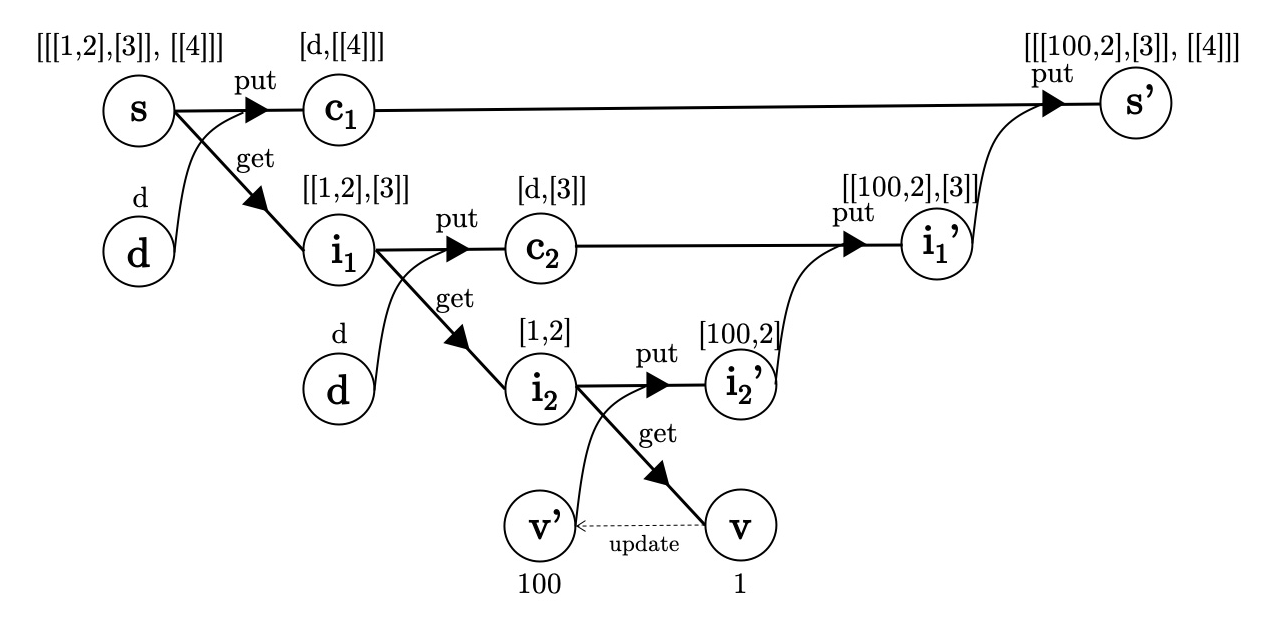
\includegraphics[height=5cm]{./fig/fig3.eps}
  \vspace{-0.25cm}
  \caption{Evaluating $phead \ \tilde{\circ} \ phead \ \tilde{\circ} \ phead$ by keeping complements}
  \vspace{-0.5cm}
  \label{fig:eval-comp-phead-2}
\end{figure}


In this paper, we make the first attempt for seriously considering the efficiency of evaluating BX compositions, and
solve the problem by introducing two methods based on memoization to gain fast evaluation for (left associative) BX compositions.
The first method uses straightforward memoization: ``keeping \emph{intermediate states in a table} and using them when needed''. This avoids repeated $get$ computations and improves the runtime in many cases. However, this simple memoization needs to keep and search values in a table, which may introduce big cost for large inputs. We explain this method in Section~\ref{sect:minbigulm}.

To treat large inputs, we propose the second method based on memoization: ``keeping \emph{complements in a closure} and using them when needed''.
\textcolor{red}{Here, complements are information from sources that makes $get$ injective, which is in turn needed to evaluate $put$.
  In the middle $put$ and $get$ of Figure \ref{fig:eval-comp-phead},
  we use $i_1$, $[[1,2],[3]]$ and $i_2'$, $[100,2]$ to obtain the updated source $[[100,2],[3]]$. However, $[1,2]$ is simply replaced by $[100,2]$ and not used to construct the result of $put$. In this case we can use $[..., [3]]$ as a complement.}
The key idea of the second approach is straightforward: Complements are smaller
% program fragments
than
% the original
intermediate states.
%Therefore this strategy solves the previous two problems.
%Readers might already know that it is a hard problem to obtain complements in general. In our work, thanks to the following finding, it is not hard:
%
%\vspace{2mm}
%In very-well behaved \cite{Foster:2007:CBT:1232420.1232424} BX,% programs,
%$put$ is a complement function for $get$.
%, $get$ can be a complement function for $put$.
%\vspace{2mm}
%
For obtaining complements, we tuple $put$ and $get$, and produce a new function $pg$. Because $put$ produces new complements for $get$, we can shrink the size.
Let us reconsider our example $phead~\tilde{\circ}~phead~\tilde{\circ}~phead$ in Figure \ref{fig:eval-comp-phead-2}, where $c_1$ and $c_2$ are complements and $d_1$ and $d_2$ are valid views for $s$ and~$i_1$. Here, two points are worth noting. First, after evaluating the leftmost $pg$, the original source $s$ need not be kept because its complete contents are in $c_1$ and~$i_1$. Second, the complements are smaller than the intermediate states in Figure~\ref{fig:eval-comp-phead}.
%This evaluation looks better than previous two strategies: this does not require repeated evaluation and require smaller storage than the original sources.
Actually, this simple
% combined
$pg$ alone is not yet effective for left associative compositions because it requires two more $put$s, which can be seen on the right side of Figure \ref{fig:eval-comp-phead-2}. To achieve an efficient evaluation, we combine two techniques, lazy update and lazy evaluation. We explain this second method and all optimizations in Section~\ref{sect:xpg}.

Both methods have been fully implemented for \emph{minBiGUL}, a core bidirectional language, which is a subset of the full bidirectional language \emph{BiGUL}. The experimental results show that our methods are much faster than the original evaluation strategy.
We give detailed experimental results in Section~\ref{sect:experiments}, discuss related work in Section~\ref{sect:related}, and conclude in Section~\ref{sect:conclusion}.

Although we will introduce the basics of bidirectional transformation in the next session, it is not complete due to space limitations. Please refer BiGUL papers \cite{Ko:2016:BFV:2847538.2847544, Ko:2017:ABB:3177123.3158129} for the details if needed.

%Due to space limitations, we assume the reader is familiar with the basic concepts of bidirectional transformation.


%The contributions of this paper are the following.

%\begin{itemize}
%\item This is the first attempt for seriously considering efficiency of evaluation of BX compositions. Our methods are better than or similar to the results by the original method in BiGUL for all test cases.
%\item We show that memoization is effective for achieving evaluation efficiency in BX languages.
%\item In BX, as far as authors know optimization by $get$ and $put$ more tight is the first attempt.
%\item Although we focus on a BX language BiGUL in this paper, these techniques can be potentially used in other BX languages.
  % \begin{itemize}
    % Although the first strategy is implemented in BiGUL, the second and third strategies are introduced by this paper.
%  \item Thanks to introduction of the strategies, it is possible to compare the evaluation strategies.
%  \item Improvement of evaluation efficiency
%  \end{itemize}
%\item Approaches used in strategy 3
%  \begin{itemize}
%  \item
% \item Optimization tequniques by tupling, and lazy update
%  \item These tequniques can be potentially used in other BX languages
%  \end{itemize}
%\end{itemize}


\newpage

\section{Bidirectional Programming Language: minBiGUL} \label{sect:minbigul}

minBiGUL, our target language in this paper, is a subset of BiGUL which is a simple yet powerful putback-based bidirectional language. BiGUL supports two transformations: a forward transformation $get$ producing a view from a source and a backward transformation $put$ taking a source and a modified view to produce an updated source. Intuitively, if we have a BiGUL program $bx$, these two transformations are following functions:

 \smallvspace
    $\qtab \getbxinline{bx} : s \to v, \quad \putbxinline{bx} : s * v \to v$
 \smallvspace
 
BiGUL is well-behaved \cite{Pacheco:2014:MCP:2543728.2543737} since two functions $\putbxinline{bx}$ and $\getbxinline{bx}$ satisfy the round-trip laws as follows:

\smallvspace
    $\qtab \putbx{bx}{s}{(\getbx{bx}{s})} = s \qquad [\textsc{GetPut}]$
    
    $\qtab \getbx{bx}{(\putbx{bx}{s}{v})} = v \qquad [\textsc{PutGet}]$
\smallvspace

The \textsc{GetPut} law means that if there is no change to the view, there should be no change to the source. The \textsc{PutGet} law means that we can recover the modified view by applying the forward transformation to the updated source.

minBiGUL inherited from BiGUL also supports transformations $put$ and $get$ which satisfy two above laws. In addition, we restrict `adaptive case's of BiGUL on minBiGUL. Then $put$ and $get$ satisfy one more law, \textsc{PutPut} \cite{Foster:2007:CBT:1232420.1232424}, like the following:

\smallvspace
$\qtab \putbx{bx}{(\putbx{bx}{s}{v'})}{v} = \putbx{bx}{s}{v} \qquad [\textsc{PutPut}]$
\smallvspace

The \textsc{PutPut} law means that a source update should overwrite the effect of previous source updates. Due to the satisfaction of three laws, \textsc{GetPut}, \textsc{PutGet} and \textsc{PutPut}, minBiGUL is very well-behaved \cite{Foster:2007:CBT:1232420.1232424}.

\subsection{Syntax}

The syntax of minBiGUL is briefly written as follows:

\smallvspace
    $bx := Skip \ h \
        | \ Replace \
        | \ Prod \ bx_1 \ bx_2 \
        | \ RearrS \ f_1 \ f_2 \ bx \
        | \ RearrV \ g_1 \ g_2 \ bx \\
    \qtabs{2} | \ Case \ cond_{sv} \ cond_{s} \ bx_1 \ bx_2 \
        | \ Compose \ bx_1 \ bx_2$
\smallvspace
        
A minBiGUL program may be either a skip of a function or a replacement or a product of two minBiGUL programs or a source/view rearrangement or a case combinator without adaptive cases or a composition of some minBiGUL programs. We use numbers, pairs and lists to construct the program inputs including the source and/or the view.

For source/view rearrangement, BiGUL uses just one lambda expression to express how to deconstruct as well as reconstruct data. It is a kind of bijection. However, to be able to implement it in OCaml, the environment used for developing minBiGUL and solutions in the paper, we need to require two functions which one is the inverse of the other. In the above syntax, $f_2 = f_1^{-1}$ and $g_2 = g_1^{-1}$.

To help make demonstration more direct, we provide the following alternatives representation: $Prod \ bx_1 \ bx_2 \equiv bx_1 \times bx_2, \ Compose \ bx_1 \ bx_2 \equiv bx_1 \circ bx_2$. In general, $\circ$ has a higher priority than $\times$. Their associativity precedence can be either left or right or mixture, but are not set by default. We need to explicitly write programs that use these operators.

\subsection{Semantics}

\begin{multicols}{2}
    \begin{definition} \label{def:minbigulput}
        $\putbx{bx}{s}{v}$

        \noindent $\putbx{Skip \ h}{s}{v} = \\
            \tab \sif{h \ s = v}{s}{\text{fail}}$
    
        \noindent $\putbx{Replace}{s}{v} = v$
    
        \noindent $\putbx{\product{bx_1}{bx_2}}{(s_1, s_2)}{(v_1, v_2)} = \\
            \tab ((\putbx{bx_1}{s_1}{v_1}),(\putbx{bx_2}{s_2}{v_2}))$
    
        \noindent $\putbx{\rearrs{f_1}{f_2}{bx}}{s}{v} = \\
            \tab f_2 \ (\putbx{bx}{(f_1 \ s)}{v})$
    
        \noindent $\putbx{\rearrv{g_1}{g_2}{bx}}{s}{v} = \\
            \tab \putbx{bx}{s}{(g_1 \ v)}$
    
        \noindent $\putbx{\casebx{cond_{sv}}{cond_{s}}{bx_1}{bx_2}}{s}{v} =\\
            \tab \text{if} \ {cond_{sv} \ s \ v} \\
            \tab \text{then} \ s' \Leftarrow \putbx{bx_1}{s}{v} \\
            \tab \text{else} \ s' \Leftarrow \putbx{bx_2}{s}{v} \\
            \tab \text{fi} \ cond_{s} \ s'; \ \text{return} \ s'$
    
        \noindent $\putbx{bx_1 \circ bx_2}{s}{v} = \\
            \tab \putbx{bx_1}{s}{(\putbx{bx_2}{(\getbx{bx_1}{s})}{v})}$
    \end{definition}
\columnbreak
    \begin{definition} \label{def:minbigulget}
        $\getbx{bx}{s}$

        \noindent $\getbx{Skip \ h}{s} = \\ 
            \tab h \ s$

        \noindent $\getbx{Replace}{s} = s$

        \noindent $\getbx{\product{bx_1}{bx_2}}{(s_1,s_2)} = \\
            \tab ((\getbx{bx_1}{s_1}),(\getbx{bx_2}{s_2}))$

        \noindent $\getbx{\rearrs{f_1}{f_2}{bx}}{s} = \\ 
            \tab \getbx{bx}{(f_1 \ s)}$

        \noindent $\getbx{\rearrv{g_1}{g_2}{bx}}{s} = \\ 
            \tab g_2 \ (\getbx{bx}{s})$

        \noindent $\getbx{\casebx{cond_{sv}}{cond_{s}}{bx_1}{bx_2}}{s} = \\
            \tab \text{if} \ {cond_{s} \ s} \\
            \tab \text{then} \ v' \Leftarrow \getbx{bx_1}{s} \\ 
            \tab \text{else} \ v' \Leftarrow \getbx{bx_2}{s} \\ 
            \tab \text{fi} \ {cond_{sv} \ s \ v'}; \ \text{return} \ v'$

        \noindent $\getbx{bx_1 \circ bx_2}{s} = \\ 
            \tab \getbx{bx_2}{(\getbx{bx_1}{s})}$
    \end{definition}
\end{multicols}

We define the semantics of $put$ and $get$ as in Definitions~\ref{def:minbigulput} and \ref{def:minbigulget} respectively. Instead of using $v'$ in the $put$ direction like Figures~\ref{fig:eval-phead}, \ref{fig:eval-comp-phead} and \ref{fig:eval-comp-phead-2}, we just simply use notation $v$ as the updated view. The later definitions also follow this convention.

In the above definitions, we use if-then-else-fi statements to express semantics of $\putbxinline{Case}$ and $\getbxinline{Case}$ where $\Leftarrow$ means assignments. This statement is useful to describe many functions related to $Case$ in this paper. Statement (if $E_1$ then $X_1$ else $X_2$ fi $E_2$) means ``if the test $E_1$ is true, the statement $X_1$ is executed and the assertion $E_2$ must be true, otherwise, if $E_2$ is false, the statement $X_2$ is executed and the assertion $E_2$ must be false.'' If the values of $E_1$ and $E_2$ are distinct, the if-then-else-fi structure is undefined. We can write the equivalent if-then-else statement as follows:

\smallvspace
$\tab \text{if } E_1 \text{ then } X_1 \text{ else } X_2 \text{ fi } E_2; S\\
\tabs{2} \ \equiv \text{if }E_1 = true \text{ then } \{ X_1; \text{ if } E_2 = true \text{ then } S \text{ else } undefined \}\\
    \tabs{4} \text{else } \{ X_2; \text{ if } E_2 = false \text{ then } S \text{ else } undefined \}$
\smallvspace
    
\noindent As an example of minBiGUL program, consider the definition of $phead$ :\\
\smallvspace
$\tab phead = RearrS \ f_1 \ f_2 \ bx_s \ \text{where: } f_1 = \lambda (s::ss).(s,ss), \, f_2 = \lambda (s,ss).(s::ss),\\
    \qtab bx_s = RearrV \ g_1 \ g_2 \ bx_v \ \text{where: } g_1 = \lambda v.(v,()), \, g_2 = \lambda (v,()).v,\\
        \qtabs{2} bx_v = \product{Replace}{(Skip \ (\lambda \_.())}$
\smallvspace
        
The above program rearranges the source, a non-empty list, to a pair of its head element $s$ and its tail $ss$, and the view to a pair $(v, ())$, then we can use $v$ to replace $s$ and $()$ to keep $ss$. Intuitively, $\putbx{phead}{s_0}{v_0}$ returns a list whose head is $v_0$ and tail is the tail of $s_0$, and $\getbx{phead}{s_0}$ returns the head of the list $s_0$. For instance, $\putbx{phead}{[1,2,3]}{100} = [100,2,3]$ and $\getbx{phead}{[1,2,3]} = 1$. If we want to update the head element of the head element of a list of lists by using the view, we can define a composition like $phead \circ phead$. For example:

\smallvspace
$\tab \putbx{phead \circ phead}{[[1,2,3],[\,],[4,5]]}{100} = [[100,2,3],[\,],[4,5]]$

$\tab \getbx{phead \circ phead}{[[1,2,3],[\,],[4,5]]} = 1$
\smallvspace

In the end of this section, let us see the minBiGUL definition of $bfoldr$ which is a putback function of an important higher-order function on lists, $foldr$:

\smallvspace
$\tab bfoldr \ bx = Case \ cond_{sv} \ cond_s \ bx_1 \ bx_2$ where:\\
$\tabs{3} \ cond_{sv} = \lambda (s_1,s_2).\lambda v.(s_1 = [\ ]), \ cond_s = \lambda (s_1,s_2).(s_1 = [\ ])$\\
$\tabs{3} \ bx_1 = RearrV \ g_1 \ g_2 \ bx_v$ where: \\
    $\tabs{4} g_1 = g_2^{-1} = \lambda [v].(v,[\ ]), bx_v = (Skip \ (\lambda \_.())) \times Replace$\\
$\tabs{3} \ bx_2 = RearrS \ f_1 \ f_2 \ bx_s$ where:\\
    $\tabs{4} f_1 = f_2^{-1} = \lambda ((x:xs),e).(x,(xs,e))$, 
$bx_s = ((Replace \times bfoldr \ bx) \circ bx)$
\smallvspace

\noindent In $bfoldr$, the composition is inherently left associative, and the number of composition is dynamically determined by the length of the source list. Since $\circ$ has a higher priority than $\times$, it is seemingly impossible to transform $bfoldr$ from the left associative composition style to the right one. 
%will look like a composition of many programs at some points in the evaluation if we slow down this process. Since $\circ$ has a higher priority than $\times$, it is seemingly impossible to transform $bfoldr$ from the left associative composition style to the right one. 


\section{pg}
\subsection{Self-inverse function: pg}

In minBiGUL or even BiGUL, when evaluating a composition of many programs, $get$s are re-evaluated so many times since no intermediate state is stored during the evaluation. This is a kind of information loss. One question is whether it is possible to calculate such programs without losing information. And the answer is yes. It comes from the the idea of reversible computation where all information during the evaluation need to be kept. In minBiGUL, we can do that by tupling $put$ and $get$. A pair of a source and a view is accepted as the input of a function named $pg$ to produce a new pair that contains the actual result of the corresponding minBiGUL program.

\begin{definition}
    $\pg{bx}{s}{v} = (\putbx{bx}{s}{v}, \getbx{bx}{s})$
\end{definition}

$pg$ is an involution that is self-inverse. An involution is a function $f$ that satifies $f(f(x)) = x \text{ for all } x \text{ in the domain of } f$.

\begin{proof}
$pg [\![bx]\!] \ (\pg{bx}{s}{v}) \\
    \tab = \pg{bx}{(\putbx{bx}{s}{v})}{(\getbx{bx}{s})} \quad [pg \text{ definition}] \\
    \tab = (put \ [\![bx]\!] \ (\putbx{bx}{s}{v}) \ (\getbx{bx}{s}), \getbx{bx}{(\putbx{bx}{s}{v})})  \quad [pg \text{ definition}] \\
    \tab = (put \ [\![bx]\!] \ (\putbx{bx}{s}{v}, \getbx{bx}{s}), v) \quad [\textsc{PutGet}] \\
    \tab = (put \ [\![bx]\!] \ (s, \getbx{bx}{s}), v) \quad [\textsc{PutPut}] \\
    \tab = (s, v) \quad [\textsc{GetPut}]$
\end{proof}

\subsection{Construction of pg}

$\tab \pg{Skip \ h}{s}{v} \overset{1}{=} (\sif{h \ s = v}{s}{\text{fail}}, h \ s) \\
    \qtab \overset{2}{=} \sif{h \ s = v}{(s, h \ s)}{\text{fail}} \\
    \qtab \overset{3}{=} \sif{h \ s = v}{(s, v)}{\text{fail}}$\\
There is a trick in the construction of $\pginline{Skip \ h}$. The first equality is simply based on the definitions of $pg$, $\putbxinline{Skip \ h}$ and $\getbxinline{Skip \ h}$. The second one tuples two results of $put$ and $get$ in the body of the if-expression. And the last one is quite obivious. What we call the trick here is in the second equality where in some cases, the result of $pg$ may be fail although there is no fail when evaluating $\getbxinline{Skip \ h}$.

$\tab \pg{Replace}{s}{v} = (v, s)$\\
$\tab \pg{\product{bx_1}{bx_2}}{(s_1,s_2)}{(v_1,v_2)}\\
    \qtab \overset{1}{=} ((\putbx{bx_1}{s_1}{v_1}),(\putbx{bx_2}{s_2}{v_2}), (\getbx{bx_1}{s_1}), (\getbx{bx_2}{s_2})) \\
    \qtab \overset{2}{=} (s_1, v_1) \Leftarrow \pg{bx_1}{s_1}{v_1}; \\
        \qtab \tab \ \, (s_2, v_2) \Leftarrow \pg{bx_2}{s_2}{v_2}; \\
        \qtabs{2} ((s_1,s_2), (v_1,v_2))$\\
$\tab \pg{\rearrs{f_1}{f_2}{bx}}{s}{v} \overset{1}{=} (f_2 \ (\putbx{bx}{(f_1 \ s)}{v}), \getbx{bx}{(f_1 \ s)}) \\
    \qtab \overset{2}{=} (s, v) \Leftarrow \pg{bx}{f_1 \ s}{v};\\
        \qtabs{2} (f_2 \ s, v)$\\
$\tab \pg{\rearrv{g_1}{g_2}{bx}}{s}{v} \overset{1}{=} (\putbx{bx}{s}{(g_1 \ v)}, g_2 \ (\getbx{bx}{s})) \\
    \qtab \overset{2}{=} (s, v) \Leftarrow \pg{bx}{s}{g_1 \ v}; \\
        \qtabs{2} (s, g_2 \ v)$\\
Constructions of $pg$ for the replacement, the product and the source/view rearrangements are very clear when just paring $put$ and $get$ respectively, then doing basic changes.

$\tab \pg{\casebx{cond_{sv}}{cond_{s}}{bx_1}{bx_2}}{s}{v} \\
\tabs{2} \overset{1}{=} (\text{if} \ {cond_{sv} \ s \ v} \qtabs{3} \tab \overset{2}{=} \text{if} \ {cond_{sv} \ s \ v} \ \&\& \ {cond_{s} \ s} \\
\tab \qtab \text{then} \ s' \Leftarrow \putbx{bx_1}{s}{v} \qtabs{2} \, \text{then} \ (s', v') \Leftarrow \pg{bx_1}{s}{v}\\
\tab \qtab \text{else} \ s' \Leftarrow \putbx{bx_2}{s}{v} \qtabs{2} \ \, \text{else} \ (s', v') \Leftarrow \pg{bx_2}{s}{v}\\
\tab \qtab \text{fi} \ cond_{s} \ s'; \text{ return } s', \qtabs{2} \tab \ \, \text{fi} \ cond_{s} \ s' \ \&\& \ cond_{sv} \ s \ v'; \text{ return } (s',v')\\
\tab \qtab \quad \text{if} \ {cond_{s} \ s}\\
\tab \qtab \quad \text{then} \ v' \Leftarrow \getbx{bx_1}{s}\\
\tab \qtab \quad \text{else} \ v' \Leftarrow \getbx{bx_2}{s}\\
\tab \qtab \quad \text{fi} \ {cond_{sv} \ s \ v'}; \text{ return } v')$

A restriction for $\pginline{Case}$ needs to be introduced here. We know that there is one entering condition and one exit condition when evaluating $\putbxinline{Case}$ as well as $\getbxinline{Case}$. If a tupling $put$ and $get$ occurs, there will be 4 combinations of these conditions. This means that two entering conditions of $\putbxinline{Case}$ and $\getbxinline{Case}$ are not always simultaneously satified. The evaluated branches are distinct in the $put$ and $get$ directions for combinations $((cond_{sv} \ s \ v) \ \&\& \ (not (cond_{s} \ s)))$ and $((not (cond_{sv} \ s \ v) \ \&\& \ (cond_{s} \ s))$, which are restricted in this paper. This does not happen for the others which is used in the construction of $\pginline{Case}$.

$\tab \pg{bx_1 \circ bx_2}{s}{v} \\
    \tabs{2} \overset{1}{=} (\putbx{bx_1}{s}{(\putbx{bx_2}{(\getbx{bx_1}{s})}{v})}, \getbx{bx_2}{(\getbx{bx_1}{s})}) \\
    \tabs{2} \overset{2}{=} v_1 \Leftarrow \getbx{bx_1}{s}; \qtabs{3} \ \, \overset{3}{=} (s_1, v_1) \Leftarrow \pg{bx_1}{s}{dummy};\\
        \tab \qtab (s_2, v_2) \Leftarrow \pg{bx_2}{v_1}{v}; \qtabs{2} (s_2, v_2) \Leftarrow \pg{bx_2}{v_1}{v};\\
        \tab \qtab (s_3, v_3) \Leftarrow \pg{bx_1}{s}{s_2}; \qtabs{2} (s_3, v_3) \Leftarrow \pg{bx_1}{s}{s_2};\\
            \qtab \tabs{2} (s_3, v_2) \qtabs{6} (s_3, v_2)\\
    \tabs{2} \overset{4}{=} (s_1, v_1) \Leftarrow \pg{bx_1}{s}{construct\_dummy \ s}; \\
        \tab \qtab (s_2, v_2) \Leftarrow \pg{bx_2}{v_1}{v}; \\
        \tab \qtab (s_3, v_3) \Leftarrow \pg{bx_1}{s_1}{s_2}; \\
            \qtab \tabs{2} (s_3, v_2)$

The construction of $\pginline{bx_1 \circ bx_2}$ can be considered as the soul of the $pg$ function. The first two equalities comes from mentioned definitions and some basic transformations. The third one rewrites $v_1 \Leftarrow \getbx{bx_1}{s}$ into $(s_1, v_1) \Leftarrow \pg{bx_1}{s}{dummy}$. It is possible if we consider $\getbx{bx_1}{s}$ as the second element of $\pg{bx_1}{s}{dummy}$ where $dummy$ is a special value that makes the $put \, [\![bx_1]\!]$ valid. Due to \textsc{GetPut} law, we can use $get \ s$ to update the source $s$ in the $put$ direction. Then it is feasible to construct a $dummy$ from the source. The last equality changes $dummy$ by an application $construct\_dummy \ s$, and also substitutes $s$ in $(s_3, v_3) \Leftarrow \pg{bx_1}{s}{s_2}$ by $s_1$ which is the evaluated result of $\putbx{bx_1}{s}{(construct\_dummy \ s)}$. This transformation is possible because of the \textsc{PutPut} law. Then, $v_3$ in the result pair $(s_3,v_3)$ equals $dummy$. So we can realize that there is no loss information when computing a composition.

\section{cpg}

When evaluating $\pginline{bx_1 \circ bx_2}$, we realize that there are three $pg$ calls, of which twice for $\pginline{bx_1}$ and once for $\pginline{bx_2}$. If a given program is a left-associative composition, the number of $pg$ calls will be exponential. Therefore, the runtime inefficiency is inevitable. In this section, we introduce a new function, $cpg$, accumulates changes in the source and the view to solve that problem. $\cpg{bx}{ks}{kv}{s}{v}$ is an extension of $\pg{bx}{s}{v}$ where $ks$ and $kv$ are continuations used to hold the modification information, and $s$ and $v$ are used to keep evaluated values. The output of this function is a 4-tuple $(ks, kv, s, v)$.

To be more convenient for presenting the definition of $cpg$ as well as the other functions later, we provide some following utility functions:

$\tab fst = \lambda (x_1,x_2). x_1 \qtab snd = \lambda (x_1,x_2). x_2\\
 \tab con = \lambda ks_1. \lambda ks_2. \lambda x. ((ks_1 \ x),(ks_2 \ x))$

\begin{definition}
$\cpg{bx}{ks}{kv}{s}{v}$

$\cpg{Skip \ h}{ks}{kv}{s}{v} = \text{ if } h \ s = v \text{ then } (ks, kv, s, v) \text{ else fail}$

$\cpg{Replace}{ks}{kv}{s}{v} = (kv, ks, v, s)$

$\cpg{\product{bx_1}{bx_2}}{ks}{kv}{s}{v} =\\
    \tab (ks_1, kv_1, s_1, v_1) \Leftarrow \cpg{bx_1}{fst \circ ks}{fst \circ kv}{fst \ s}{fst \ v};\\
    \tab (ks_2, kv_2, s_2, v_2) \Leftarrow \cpg{bx_2}{snd \circ ks}{snd \circ kv}{snd \ s}{snd \ v};\\
    \qtab (con \ ks_1 \ ks_2, con \ kv_1 \ kv_2, (s_1,s_2), (v_1,v_2))$

$\cpg{RearrS \ f_1 \ f_2 \ bx}{ks}{kv}{s}{v} =\\
    \tab (ks, kv, s, v) \Leftarrow \cpg{bx}{f_1 \circ ks}{kv}{f_1 \ s}{v};\\
    \qtab (f_2 \circ ks, kv, s, v)$

$\cpg{RearrV \ g_1 \ g_2 \ bx}{ks}{kv}{s}{v} =\\
    \tab (ks, kv, s, v) \Leftarrow \cpg{bx}{ks}{g_1 \circ kv}{s}{g_1 \ v};\\
    \qtab (ks, g_2 \circ kv, ks, g_2 \ v)$

$\cpg{Case \ cond_{sv} \ cond_{s} \ bx_1 \ bx_2}{ks}{kv}{s}{v} =\\
    \tab \text{if} \ cond_{sv} \ s \ v \ \&\& \ cond_{s} \ s\\
    \tab \text{then} \ (ks, kv, s', v') \Leftarrow \cpg{bx_1}{ks}{kv}{s}{v}\\
    \tab \text{else} \ (ks, kv, s', v') \Leftarrow \cpg{bx_2}{ks}{kv}{s}{v}\\
    \tab \text{fi} \ cond_{s} \ s' \ \&\& \ cond_{sv} s v'; \ \text{return} \ (ks, kv, s', v')$

$\cpg{bx_1 \circ bx_2}{ks}{kv}{s}{v} =\\
    \tab (ks_1, kv_1, s_1, v_1) \Leftarrow \cpg{bx_1}{ks}{id}{s}{construct\_dummy \ s};\\
    \tab (ks_2, kv_2, s_2, v_2) \Leftarrow \cpg{bx_2}{kv_1}{kv}{v_1}{v};\\
        \qtab (ks_1 \circ ks_2, kv_2,  ks_1 \ s_2, v_2)$
\end{definition}

Apart from the last construction, the others are quite similar to the corresponding ones of $pg$, but have some updates over the source and the view on accumulative functions $ks$ and $kv$ respectively.\\
For $\cpginline{bx_1 \circ bx_2}$, there are only two $cpg$ calls. The first call $\cpginline{bx_1}$ requires parameter $(ks, id, s, construct\_dummy \ s)$ where $s$ and $ks$ are corresponding to the source and the update over source. Because there is no real view here, we need to construct a dummy from the source. Then the continuation updating on this dummy should be initiated as an identity function. The first $cpg$ call is assigned to a 4-tuple $(ks_1, kv_1, s_1, v_1)$ where $s_1$ is redundant because it is not used in the later evaluation process. Some computations to get $s_1$ are seen as redundant. Such values and computations have negative impacts on the runtime as well as the memory allocation in the system. In the next assigment, a 4-tuple $(ks_2, kv_2, s_2, v_2)$ is assigned by the second $cpg$ call which uses the input as $(kv_1, kv, v_1, v)$ where $kv_1$ and $v_1$ are obtained from the result of the first assignment, and $kv$ and $v$ come from the input. It is relatively similar to the second $pg$ call assignment in $\pginline{bx_1 \circ bx_2}$. After two $cpg$ calls, a function application, $ks_1 \ s_2$, is used to produce the updated source instead of calling $\cpginline{bx_1}$ one more time like in $\pginline{bx_1 \circ bx_2}$.\\
Suppose that we have a source $s_0$ and a view $v_0$. The pair of the updated source and view $(s, v)$ where $s = \putbx{bx}{s_0}{v_0}$ and $v = \getbx{bx}{s_0}$ can be obtained using $cpg$ as follows:\\
    $\tab s \Leftarrow s_0; v \Leftarrow v_0; (ks, kv, s, v) \Leftarrow \cpg{bx}{\lambda \_.s}{id}{s}{v};\\
        \qtab (s; v)$\\
In general, the begining of a continuation should be an identity function. However, to be able to use the function application to get the result of $\cpginline{bx_1 \circ bx_2}$, the accumulative function on the source $s$ needs to be initiated as a constant function $\lambda \_.s$.\\
Suppose the begining of continuations $ks$ and $kv$ are $ks_0$ and $id$ respectively. Let's consider $\cpg{phead_1 \circ phead_2}{ks_0}{id}{s}{v}$ where $s = [[1,2,3], [\,], [4,5]]$ and $v = 100$. After the first two assignments in the definition of $cpg$ for the composition, we have: $ks_1 = f_2 \circ (con \ (fst \circ g_1 \circ id) \ (snd \circ f_1 \circ ks_0))$ and $s_2 = [100,2,3]$ where $f_1 = \lambda (s::ss).(s,ss)$, $f_2 = \lambda (s,ss).(s::ss)$, $g_1 = \lambda v.(v,())$. \\
Then: $ks_1 \ s_2 = (f_2 \circ (con \ (fst \circ g_1 \circ id) \ (snd \circ f_1 \circ ks_0))) \ s_2 \\
\tab = f_2 \ (\ (fst(g_1(id(s_2))) \ , \ snd(f_1(ks_0(s_2))))\ )\\
\tab = fst(g_1(id(s_2))) :: snd(f_1(ks_0(s_2))) = [100,2,3] :: snd(f_1(ks_0([100,2,3])))$\\
If $ks_0$ is an identity function, $ks_1 \ s_2 = [100,2,3] :: [2,3]$. This is an unexpected result when we target it to be the updated source. If $ks_0 = \lambda \_.s$ where $s = [[1,2,3], [\,], [4,5]]$, $ks_1 \ s_2 = [100,2,3] :: [[\,], [4,5]] = [[100,2,3], [\,], [4,5]]$. This time, the result is what we want to see. Through the above example, using the continuation $ks$ as a constant function at the beginning contributes to keep the unchanged parts in the source.

\section{kpg}

In the previous section, we have known that there are some variables which are evaluated but not used later when evaluating $\cpginline{bx_1 \circ bx_2}$. Now we introduce $kpg$, an extension of $cpg$, for keeping away such redundant computations. 
While $cpg$ evaluate values eagerly, $kpg$ does the opposite. Every values are evaluated lazily in a computation of $kpg$. The input of $\kpginline{bx}$ is expanded to a 6-tuple $(ks, kv, ks', kv', s, v)$ where $ks$ and $kv$ keep the modifcation information, $s$ and $v$ hold evaluated values, and $ks'$ and $kv'$ are used for lazy evaluation of actual values. The output of this function is also a 6-tuple $(ks, kv, ks', kv', s, v)$.\\
Suppose that we have a source $s_0$ and a view $v_0$. The pair of the updated source and view $(s, v)$ where $s = \putbx{bx}{s_0}{v_0}$ and $v = \getbx{bx}{s_0}$ can be obtained using $kpg$ as follows:\\
    $\tab s \Leftarrow s_0; v \Leftarrow v_0; (ks, kv, ks', kv', s, v) \Leftarrow \kpg{bx}{\lambda \_.s}{id}{id}{id}{s}{v};\\
        \qtab (ks' \ s; kv' \ v)$\\
The begining of accumulative functions $ks'$ and $kv'$ are set as identity, while $ks$ and $kv$ are initiated as the same with the corresponding ones in $cpg$.

\begin{definition}
$\kpg{bx}{ks}{kv}{ks'}{kv'}{s}{v}$

$\kpg{Skip \ h}{ks}{kv}{ks'}{kv'}{s}{v} =\\
    \tab s \Leftarrow ks' \ s; \quad v \Leftarrow kv' \ v; \quad ks' \Leftarrow id; \quad kv' \Leftarrow id;\\
    \tab \text{if} \ h \ s = v \ \text{then} \ (ks, kv, ks', kv', s, v) \ \text{else fail}$

$\kpg{Replace}{ks}{kv}{ks'}{kv'}{s}{v} = (kv, ks, kv', ks', v, s)$

$\kpg{\product{bx_1}{bx_2}}{ks}{kv}{ks'}{kv'}{s}{v} =\\
    \tab s \Leftarrow ks' \ s; \quad v \Leftarrow kv' \ v; \quad ks' \Leftarrow id; \quad kv' \Leftarrow id;\\
    \tab (ks_1, kv_1, ks_1', kv_1', s_1, v_1) \Leftarrow \kpg{bx_1}{fst \circ ks}{fst \circ kv}{fst \circ ks'}{fst \circ kv'}{s}{v};\\
    \tab (ks_2, kv_2, ks_2', kv_2', s_2, v_2) \Leftarrow \kpg{bx_2}{snd \circ ks}{snd \circ kv}{snd \circ ks'}{snd \circ kv'}{s}{v};\\
    \qtab ( con \ ks_1 \ ks_2, con \ kv_1 \ kv_2, con \ (ks_1' \circ fst) \ (ks_2' \circ snd),\\
    \qtab con \ (kv_1' \circ fst) \ (kv_2' \circ snd), \\
    \qtab (s_1, s_2), (v_1,v_2))$

$\kpg{RearrS \ f_1 \ f_2 \ bx}{ks}{kv}{ks'}{kv'}{s}{v} =\\
    \tab (ks, kv, ks', kv', s, v) \Leftarrow \kpg{bx}{f_1 \circ ks}{kv}{f_1 \circ ks'}{kv'}{s}{v};\\
    \qtab (f_2 \circ ks, kv, f_2 \circ ks', kv', s, v)$

$\kpg{RearrV \ g_1 \ g_2 \ bx}{ks}{kv}{ks'}{kv'}{s}{v} =\\
    \tab (ks, kv, ks', kv', s, v) \Leftarrow \kpg{bx}{ks}{g_1 \circ kv}{ks'}{g_1 \circ kv'}{s}{v};\\
    \qtab (ks, g_2 \circ kv, ks', g_2 \circ kv', s, v)$

$\kpg{Case \ cond_{sv} \ cond_{s} \ bx_1 \ bx_2}{ks}{kv}{ks'}{kv'}{s}{v} =\\
    \tab s \Leftarrow ks' \ s; \quad v \Leftarrow kv' \ v; \quad ks' \Leftarrow id ; \quad kv' \Leftarrow id;\\
    \tab \text{if} \ cond_{sv} \ s \ v \&\& \ cond_{s} \ s\\
    \tab \text{then} \ (ks, kv, ks', kv', s', v') \Leftarrow \kpg{bx_1}{ks}{kv}{ks'}{kv'}{s}{v}\\
    \tab \text{else} \ (ks, kv, ks', kv', s', v') \Leftarrow \kpg{bx_2}{ks}{kv}{ks'}{kv'}{s}{v}\\
    \tab \text{fi} \ cond_s \ (ks' \ s') \ \&\& \ cond_{sv} \ s \ (kv' \ v'); \ \text{return} \ (ks, kv, ks', kv', s', v')$

$\kpg{bx_1 \circ bx_2}{ks}{kv}{ks'}{kv'}{s}{v} =\\
    \tab (ks_1, kv_1, \underline{ks_1'}, kv_1', \underline{s_1}, v_1) \Leftarrow \kpg{bx_1}{ks}{id}{ks'}{id}{s}{construct\_dummy \ s};\\
    \tab (ks_2, kv_2, ks_2', kv_2', s_2, v_2) \Leftarrow \kpg{bx_2}{kv_1}{kv}{kv_1'}{kv'}{v_1}{v};\\
    \qtab (ks_1 \circ ks_2, kv_2, ks_1 \circ ks_2', kv_2', s_2, v_2)$
\end{definition}

In the construction of $kpg$, $s$ and $v$ hold actual values only in case of $Skip$ and $Case$. Except them, the functions for computation will be kept in $ks'$ and $kv'$. When evaluating $\kpginline{bx_1 \circ bx_2}$, $ks_1'$ and $s_1$ in the result of the first assignment are still redundant but they are not evaluated. In $\kpginline{bx_1 \ prod \ bx_2}$, the evaluation of $ks'$ and $kv'$ will be done indendently in two assingments using $\kpginline{bx_1}$ and $\kpginline{bx_2}$. There may be some recomputations in $fst \circ ks'$ and $snd \circ ks'$ as well as $fst \circ kv'$ and $snd \circ kv'$. It is possible to evaluate actual values in $s$ and $v$ before calling $\kpginline{bx_1}$ to remove the redundancy like that.

\section{xpg}
So far, when computing a composition, we only recursively call an unique function, either $pg$ or $cpg$ or $kpg$. To be more flexible, we make a new extension, $xpg$, allowing to call external functions.

\begin{definition}
$\xpg{bx}{s}{v}$

$\xpg{bx}{s}{v} = \text{same with } pg \text{ if } bx \neq bx_1 \circ bx_2$

$\xpg{bx_1 \circ bx_2}{s}{v} =\\
    \tab (ks_1,kv_1, ks_1', kv_1', s_1, v_1) \Leftarrow \kpg{bx_1}{\lambda \_.s}{id}{id}{id}{s}{construct\_dummy \ s};\\
    \tab (s_2, v_2) \Leftarrow \xpg{bx_2}{kv_1' \ v_1}{v};\\
    \qtab (ks_1 \ s_2, v_2)$
\end{definition}
Similar to $pg$, $\xpginline{bx}$ accepts a pair of the source and the view $(s,v)$ to produce the new pair. The constructions of $\xpginline{bx}$ when $bx$ is not a composition are the same as the ones of $\pginline{bx}$. Note that, $xpg$ is called recursively instead of $pg$. For $\xpginline{bx_1 \circ bx_2}$, we use two function calls and a function application to calculate the result. The first call and the function application come from $kpg$ approaches, while the second call is based on $pg$ approach.

\section{Experiments (old)}

This section describes the experiments involving $minBiGUL$, $pg$, $cpg$, $kpg$ and $xpg$. The evaluation time and the memory allocation are considered in each test.

\subsection{Experiment environment \& Test cases}
We implemented 5 approaches with OCaml 4.07.1 in the same environment as follows: macOS 10.14.6, processor Intel Core i7 (2.6 GHz), RAM 16 GB 2400 MHz DDR4. The OCaml runtime system options and garbage collection parameters are set as default.

We also conducted tests on 5 cases, including many composition styles such as left or right associative, non-recursive or recursive. Table \ref{tab:test-cases} shows more details on these cases.

\begin{table}[hbt!]
    \centering
    \caption{Test cases}
    \label{tab:test-cases}
    \begin{tabular*}{\textwidth}{|c @{\extracolsep{\fill}}|l|l|l|c|c|c|c|}
        \hline
        \multirow{2}{*}{No} & \multicolumn{1}{c|}{\multirow{2}{*}{Name}} & \multicolumn{1}{c|}{\multirow{2}{*}{Associative}} & \multicolumn{1}{c|}{\multirow{2}{*}{Recursive}} & \multicolumn{2}{c|}{Input} & \multicolumn{2}{c|}{Output} \\ \cline{5-8} 
        & \multicolumn{1}{c|}{} & \multicolumn{1}{c|}{} & \multicolumn{1}{c|}{} & \multicolumn{1}{c|}{$s_0$} & \multicolumn{1}{c|}{$v_0$} & \multicolumn{1}{c|}{$s_r$} & \multicolumn{1}{c|}{$v_r$} \\ \hline
        1 & lassoc-comp-replace & left & no & 1 & 100 & 100 & 1 \\ \hline
        2 & rassoc-comp-replace & right & no & 1 & 100 & 100 & 1 \\ \hline
        3 & lassoc-comp-phead & left & no & $\underbrace{[[\ldots[1]\ldots]]}_{\text{n+1 times}}$ & 100 & $\underbrace{[[\ldots[100]\ldots]]}_{\text{n+1 times}}$ & 1 \\ \hline
        4 & rassoc-comp-phead & right & no & $\underbrace{[[\ldots[1]\ldots]]}_{\text{n+1 times}}$ & 100 & $\underbrace{[[\ldots[100]\ldots]]}_{\text{n+1 times}}$ & 1 \\ \hline
        5 & breverse & left/right & yes & [1..n] & [1..n] & [n..1] & [n..1] \\ \hline
    \end{tabular*}
\end{table}

In table \ref{tab:test-cases}, $s_r$ and $v_r$ are respectively updated source and view which are produced by applying $put$ and $get$ on original source $s_0$ and original view $v_0$. This means: $s_r = \putbx{bx}{s_0}{v_0}$ and $v_r = \getbx{bx}{s_0}$, where $bx$ is one of the 5 cases mentioned in the table. Note that the results $s_r$ and $v_r$ do not depend on the associative style of the composition. The first four test cases simply use $n$ compose operators to make a composition of $n + 1$ similar $BX$ programs which are non-recursive. For example, \textit{lassoc-comp-replace}, left-associative composition of $Replace$s, looks like $(\ldots((Replace \circ Replace) \circ Replace) \circ \ldots \circ Replace) \circ Replace$, while \textit{rassoc-comp-replace}, right-associative composition of $Replace$s, is like $Replace \circ (Replace \circ (Replace \circ \ldots \circ (Replace \circ Replace)\ldots))$, where there are $n + 1 \ Replace$s in each case. The last test case, \textit{breverse}, is defined in terms of \textit{bFoldr}, a putback function for \textit{foldr} which is an important higher-order function on lists. This case is more natural than the other since \text{bFoldr} is a Case analysis whose a branch contains a composition $bx_1 \circ bx_2$ where $bx_1$ is a product of a simple function and $bFoldr$. It will look like a composition of more BX programs at some point if we slow down the evaluation. Note that $\circ$ has a higher priority than $\times$. This leads to seemingly impossible to transform \textit{bReverse} as well as \textit{bFoldr} from left-associative style to right-associative style.

\subsection{Results and discussions}

Firstly, from definitions of $put$, $cpg$, $kpg$ and $xpg$, we have No($cpg$) = No($kpg$) = No($xpg$) = No($put$) where No($f$) is the number of function call $f$. Here we consider that No($xpg$) in evaluating $\xpginline{bx_1 \circ bx_2}$ includes both the number of $kpg$s which are used in $\kpginline{bx_1}$ and the number of $xpg$s which are used in $\xpginline{bx_2}$. For right-associative and non-recursive compositions (\textit{rassoc-comp-replace} and \textit{rassoc-comp-phead}), No($get$), No($put$) and No($pg$) are linear. For left-associative and non-recursive compositions (\textit{lassoc-comp-replace} and \textit{lassoc-comp-phead}), No($put$) is still linear while No($get$) is quadratic and No($pg$) is under an exponential distribution. For recursive composition (\textit{breverse}), all three are nonlinear. The appendix will provide more complete insights about those statements. Now we take a closer look at the empirical results.

%\newcommand{\qaddplot}[1]{
    \pgfplotstableread[col sep=comma]{csv/#1.csv}\data
    \addplot table[x=nComp,y=minbigul]{\data};
    \addplot table[x=nComp,y=minbigul_m]{\data};
    \addplot table[x=nComp,y=xpg]{\data};
}

\begin{figure}
    \centering
    \begin{tikzpicture}
        \pgfplotsset{footnotesize,samples=9}
        \begin{groupplot}[
                group style = {
                    group size = 2 by 7,
                    horizontal sep = 2.5cm,
                    vertical sep = 1cm,
                }, 
                width = 4.5cm, 
                height = 3.5cm,
                % xmin = 0, xmax = 110000,
                % ymin = 0,
                scaled x ticks = false,
                x tick label style = {
                    /pgf/number format/fixed
                },
                scaled y ticks = false,
                y tick label style = {
                    /pgf/number format/fixed,
                    /pgf/number format/precision=2,
                },
                every x tick scale label/.style={at={(rel axis cs:1,0)},anchor=south west,inner sep=1pt},
                every y tick scale label/.style={at={(rel axis cs:-0.1,1.05)},anchor=south east,inner sep=1pt},
                max space between ticks=1000pt,
                try min ticks = 5,
                label style={font=\small},
                tick label style={font=\small} 
            ]

            \nextgroupplot[ 
                title = {\textit{lcomp-replace}}, 
                legend style = {legend to name = legendgroup,},
                scaled x ticks = {base 10:-5},
                scaled y ticks = {base 10:-1},
            ]
                \pgfplotstableread[col sep=comma]{csv/lcomp-replace.csv}\data
                \addplot table[x=nComp,y=minbigul]{\data}; \label{plots:put};
                \addplot table[x=nComp,y=minbigul_m]{\data}; \label{plots:put$_m$};
                \addplot table[x=nComp,y=xpg]{\data}; \label{plots:xpg};
                \coordinate (topl) at (rel axis cs:0,1);
            
            \nextgroupplot[ 
                title = {\textit{lcomp-replace-ldata}}, 
                legend style = {legend to name = grouplegend,},
                scaled x ticks = {base 10:-5},
                scaled y ticks = {base 10:-1},
            ]
                \qaddplot{lcomp-replace-ldata};
            
            \nextgroupplot [
                hide axis, xtick=\empty, ytick=\empty
            ]

            \nextgroupplot[ 
                title = {\textit{lcomp-phead-ldata}}, 
                scaled x ticks = {base 10:-5},
                scaled y ticks = {base 10:-2},
            ]
                \qaddplot{lcomp-phead-ldata};

            \nextgroupplot[
                title = {\textit{lcomp-ptail}},
                scaled x ticks = {base 10:-5},
                scaled y ticks = {base 10:-2},
            ]
                \qaddplot{lcomp-ptail};

            \nextgroupplot[
                title = {\textit{lcomp-ptail-ldata}},
                scaled x ticks = {base 10:-5},
                scaled y ticks = {base 10:-2},
            ] 
                \qaddplot{lcomp-ptail-ldata};

            \nextgroupplot[
                title = {\textit{lcomp-bsnoc}},
                scaled x ticks = {base 10:-4},
                scaled y ticks = {base 10:-2},
            ]
                \qaddplot{lcomp-bsnoc};

            \nextgroupplot[
                title = {\textit{lcomp-bsnoc-ldata}},
                scaled x ticks = {base 10:-4},
                scaled y ticks = {base 10:-2},
            ] 
                \qaddplot{lcomp-bsnoc-ldata};

            \nextgroupplot[
                title = {\textit{bmapreplace}},
                scaled x ticks = {base 10:-4},
                scaled y ticks = {base 10:-1},
            ]
                \qaddplot{bmapreplace};

            \nextgroupplot[
                title = {\textit{bmapreplace-ldata}},
                scaled x ticks = {base 10:-4},
                scaled y ticks = {base 10:-1},
            ] 
                \qaddplot{bmapreplace-ldata};

            \nextgroupplot[
                title = {\textit{breverse}},
                % xmax = 10000,
                scaled x ticks = {base 10:-5},
                scaled y ticks = {base 10:-3},
            ] 
                \qaddplot{breverse};
                % \coordinate (botl) at (rel axis cs:0,0);

            \nextgroupplot[
                title = {\textit{breverse-ldata}},
                % xmax = 10000,
                scaled x ticks = {base 10:-5},
                scaled y ticks = {base 10:-2},
                % xlabel = {number of compositions},
            ] 
                \qaddplot{breverse-ldata};
                \coordinate (botr) at (rel axis cs:1,0);
        \end{groupplot}

        \path (topl|-current bounding box.north)--
            coordinate(legendpos)
            (botr|-current bounding box.north);
        \matrix[
            matrix of nodes,
            anchor = south,
            draw,
            inner sep = 0.2em,
            draw
        ]at([yshift=1ex]legendpos) {
            \ref{plots:put} & $put$ & [2pt]
            \ref{plots:put$_m$} & $put_m$ & [2pt]
            \ref{plots:xpg} & $xpg$\\
        };

    \end{tikzpicture}

    \caption{Experimental results}
    \label{fig:result}

\end{figure}

Fig \ref{fig:result}a illustrates the evaluation times in 5 test cases. $pg$ times are always exponential for both left-associative compositions (\textit{lassoc-comp-replace}, \textit{lassoc-comp-phead}) and recursive compositions (\textit{breverse}) since No($pg$) in each case is under an exponential distribution. For left-associative and non-recursive compositions, $kpg$ times are approximate to $xpg$ times, and they are the most efficient. In case of \textit{lassoc-comp-replace}, $kpg$ time and $xpg$ time are linear, $cpg$ time and $minBiGUL$ time are nonlinear. They are quite reasonable because the data sizes are constant, No($get$) is quadractic for $minBiGUL$ while there is a linear quantity of redundant evaluations in $cpg$. In case of \textit{lassoc-comp-phead}, since the data sizes are linear and No($f$) are either linear or quadractic or exponential, all times are nonlinear. For right-associative and non-recursive compositions, $minBiGUL$, $pg$ and $xpg$ times are linear. In case of \textit{rassoc-comp-replace}, all times are small enough to consider all them as linear. In case of \textit{rassoc-comp-phead}, both $cpg$ and $kpg$ times are quadratic because the data sizes are linear and the number of redundant evaluations are also linear. For recursive compositions (\textit{breverse}), all times should be nonlinear since there is no linear number of function calls.\\
Fig \ref{fig:result}b shows the memory usage which depends on the input size and number of compositions. In general, $minBiGUL$ uses less memory than the others for non-recursive compositions (all tests except \textit{breverse}). $pg$ only uses memory efficient when handling right-associative compositions. Also for evaluating these  compositions, both $cpg$ and $kpg$ are worst in memory allocation. For recursive compositions (\textit{breverse}), $minBiGUL$ uses significantly more memory than $kpg$ as well as $xpg$.

\section{Related Work}

\begin{itemize}
    %\item BiGUL papers (PEPM, POPL, tutorial?)
    %\item the first BX paper
    %\item get-based BX
    %\item put-based BX?
    \item implementation of BX, they might have the same problem, this paper will be first attempt, semantics and correctness is considered more, but efficiency is  lacked.
    \item optimization techniques : tupling, lazy computation, fusion transformation?
    \item (view update problem paper)
\end{itemize}

\section{Conclusion and Future Work}

In this paper we focus on efficiency of composition of BX programs.
The essential finding comes from the idea of tupling: in very-well behaved BX programs we can use $put$ as a compliment function for $get$, and vice versa.
Based on the idea, we introduced $pg$, and improved it by several optimization techniques. From experimental results, our fastest approach $xpg$ is faster than other approaches for non purely right associative compositions. For right associative compositions, the original approach (miniBiGUL) is faster than $xpg$ because $xpg$ has some overhead cost. However this is not a problem, because usually programs are mix of left and right associative. If programmers know that their programs are purely right associative, they can choose miniBiGUL.

We will continue our work on the following points. First, our target language is limited to very-well behaved, because our main idea requires the put-put property. However, for practical programs, we need to extend our work to overcome the current limitations.

\begin{itemize}
\item Extend our approach -- overcome our limitations
  \begin{itemize}
  \item treat well-behaved programs -- How to treat adaptive cases
  \item In case expressions, the programs that use the different paths (put and get)
  \end{itemize}
\item How to obtain dummy?
\item Type system \& Typing -- for safety
\end{itemize}



\textcolor{red}{TODO: FIX reference, order, contents ..}

% From sample code
% 
% ---- Bibliography ----
%
% BibTeX users should specify bibliography style 'splncs04'.
% References will then be sorted and formatted in the correct style.
%
% \bibliographystyle{splncs04}
% \bibliography{mybibliography}
%
\begin{thebibliography}{8}
\bibitem{viewupdate}
F. Bancilhon and N. Spyratos. ``Update semantics of relational views''. ACM Transactions on Database Systems, 6(4):557--575, 1981.

\bibitem{BXcomp}
Anthony Anjorin, Thomas Buchmann, Bernhard Westfechtel, Zinovy Diskin, Hsiang-Shang Ko, Romina Eramo, Georg Hinkel, Leila Samimi-Dehkordi, and Albert Zündorf
``Benchmarking bidirectional transformations: Theory, implementation, application, and assessment'', Software and Systems Modeling, ??, 2019

\bibitem{tupling}
  M. Fokkinga. ``Tupling and mutumorphisms''. Squiggolist, 1(4), 1989.

\bibitem{josh_pepm}
  Hsiang-Shang Ko, Tao Zan, Zhenjiang Hu, BiGUL: A Formally Verified Core Language for Putback-Based Bidirectional Programming, ACM SIGPLAN 2016 Workshop on Partial Evaluation and Program Manipulation (PEPM 2016), pp.61--72, 2016.

\bibitem{josh_popl}
  Hsiang-Shang Ko, Zhenjiang Hu, An Axiomatic Basis for Bidirectional Programming , 45th ACM SIGPLAN Symposium on Principles of Programming Languages (POPL 2018), 2018.

\bibitem{BXtend}
  Thomas Buchmann. BXtend -- a framework for (bidirectional) model transformations. In Slimane Hamoudi,Luis Ferreira Pires, and Bran Selic, editors, Proceedings
of the 6th International Conference on Model-Driven Engineering and Software Development - Volume 1: MODELSWARD (MODELSWARD 2018), pages 336--345, 2018.

\bibitem{eMoflon}
  Erhan Leblebici, Anthony Anjorin, and Andy Sch"{u}rr. Developing eMoflon with eMoflon. In Davide Di Ruscio and Daniel Varro, editors, Theory and Practice of Model Transformations - 7th International Conference, ICMT 2014, Held as Part of STAF 2014, York, UK, 2014. Proceedings, volume 8568 of Lecture Notes in
Computer Science, pages 138–145. Springer, 2014.

\bibitem{EVL+Strace}
Leila Samimi-Dehkordi, Bahman Zamani, and Shekoufeh Kolahdouz-Rahimi. EVL+Strace: A novel bidirectional transformation approach. Information and Software
Technology, 100:47--72, 2018.

\bibitem{JTL}
Antonio Cicchetti, Davide Di Ruscio, Romina Eramo, and Alfonso Pierantonio. JTL: A bidirectional and change propagating transformation language. In Brian Malloy, Steffen Staab, and Mark van den Brand, editors, Proceedings of the Third International Conference on Software Language Engineering (SLE 2010), volume 6563 of Lecture Notes of Computer Science, pages 183--202, Springer-Verlag.
  
\bibitem{NMF}
Georg Hinkel and Erik Burger. Change propagation and bidirectionality in internal transformation DSLs. Soft-ware and Systems Modeling, 18(1):249--278, 2019.

  
\bibitem{SDMLib}
  SDMLib paper?

\bibitem{lenses}
  Lense papers?

\bibitem{tutorial}
  Tutorial paper of BiGUL
  
%\bibitem{ref_article1}
%Author, F.: Article title. Journal \textbf{2}(5), 99--110 (2016)

%\bibitem{ref_lncs_1}
%Author, F., Author, S.: Title of a proceedings paper. In: Editor,
%F., Editor, S. (eds.) CONFERENCE 2016, LNCS, vol. 9999, pp. 1--13.
%Springer, Heidelberg (2016). \doi{10.10007/1234567890}

%\bibitem{ref_book1}
%Author, F., Author, S., Author, T.: Book title. 2nd edn. Publisher,
%Location (1999)

%\bibitem{ref_proc1}
%Author, A.-B.: Contribution title. In: 9th International Proceedings
%on Proceedings, pp. 1--2. Publisher, Location (2010)

%\bibitem{ref_url1}
%LNCS Homepage, \url{http://www.springer.com/lncs}. Last accessed 4
%Oct 2017
\end{thebibliography}

% \appendix

\section{Remove?:First approach}

% We should skip this 

\begin{itemize}
\item Make put and get to be reversible. We need garbages (g) to keep lost infomation after evaluation.
\item put$_{REV}$ = s * v $\to$ s * gb
\item get$_{REV}$ = s $\to$ v * gb
\item introduce (put$_{REV}^{-1}$: s * gb $\to$ s * v) and (get$_{REV}^{-1}$:v * gb $\to$ s)
\item \textcolor{red}{(Missing part?)} Relationship between put$_{REV}$, get$_{REV}$, put$_{REV}^{-1}$, get$_{REV}^{-1}$ 
\end{itemize}

$\putrev{Skip \ h}{s}{v} =  \sif{h \ s = v}{(s, v)}{\text{fail}}$

$\putrev{Replace}{s}{v} = (v, s)$

$\putrev{\product{bx_1}{bx_2}}{(s_1 :: s_2)}{(v_1 :: v_2)} =\\
    \tab (s_1, gb_1) \Leftarrow \putrev{bx_1}{s_1}{v_1};\\
    \tab (s_2, gb_2) \Leftarrow \putrev{bx_2}{s_2}{v_2};\\
        \qtab (s_1 :: s_2, gb_1 :: gb_2)$

$\putrev{\rearrs{f_1}{f_2}{bx}}{s}{v} =\\
    \tab (s_1, gb_1) \Leftarrow \putrev{bx}{(f_1 \ s)}{v};\\
        \qtab (f_2 \ s_1, gb_1)$

$\putrev{\rearrv{g_1}{g_2}{bx}}{s}{v} =\\
    \tab (s_1, gb_1) \Leftarrow \putrev{bx}{s}{(g_1 \ v)};\\
        \qtab (s_1, gb_1)$

$\putrev{\casebx{cond_{sv}}{cond_{s}}{bx_1}{bx_2}}{s}{v} =\\
    \tab \text{if} \ cond_{sv} \ s \ v\\
    \tab \text{then} \ (s', gb) \Leftarrow \putrev{bx_1}{s}{v};\\
    \tab \text{else} \ (s', gb) \Leftarrow \putrev{bx_2}{s}{v};\\
    \tab \text{fi} \ cond_{s} \ s'; \ \text{return} \ (s', gb)$

$\putrev{bx_1 \circ bx_2}{s}{v} =\\
    \tab (s_1, gb_1) \Leftarrow \getrev{bx_1}{s};\\
    \tab (s_2, gb_2) \Leftarrow \putrev{bx_2}{s_1}{v};\\
    \tab (s_3, gb_3) \Leftarrow \putrev{bx_1}{s}{s_2} \ \text{in (* need to copy s *)}\\
        \qtab (s_3, gb_1 :: gb_2 :: gb_3)$

\vspace{5mm}

$\getrev{Skip \ h}{s} = {(h \ s, s)}$

$\getrev{Replace}{s} = (s, \textcolor{red}{\text{Nil}})$

$\getrev{\product{bx_1}{bx_2}}{(s_1 :: s_2)} = \\
    \tab (v_1, gb_1) \Leftarrow \getrev{bx_1}{s_1};\\
    \tab (v_2, gb_2) \Leftarrow \getrev{bx_2}{s_2};\\
        \qtab (v_1 :: v_2, gb_1 :: gb_2)$

$\getrev{\rearrs{f_1}{f_2}{bx}}{s}{v} =\\
    \tab (v_1, gb_1) \Leftarrow \getrev{bx}{(f_1 \ s)};\\
        \qtab (v_1, gb_1)$

$\getrev{\rearrv{g_1}{g_2}{bx}}{s}{v} =\\
    \tab (v_1, gb_1) \Leftarrow \getrev{bx}{s};\\
        \qtab (g_2 \ v_1, gb_1)$

$\getrev{\casebx{cond_{sv}}{cond_{s}}{bx_1}{bx_2}}{s} =\\
    \tab \text{if} \ cond_{s} \ s\\
    \tab \text{then} \ (v', gb) \Leftarrow \getrev{bx_1}{s};\\
    \tab \text{else} \ (v', gb) \Leftarrow \getrev{bx_2}{s};\\
    \tab \text{fi} \ cond_{sv} \ s \ v'; \ \text{return} \ (v', gb)$

$\getrev{bx_1 \circ bx_2}{s}{v} =\\
    \tab (v_1, gb_1) \Leftarrow \getrev{bx_1}{s};\\
    \tab (v_2, gb_2) \Leftarrow \getrev{bx_1}{s};\\
        \qtab (v_2, gb_1 :: gb_2)$

\textcolor{red}{If we use Rwhile for target language, we do not need to introduce inverse.}

\section{minBiGUL}
Now, let's consider the definition of $phead$ in BiGUL [?]:

$\tab phead :: Show \ s \Rightarrow BiGUL \ [s] \ s\\
\tab phead = \$(RearrS \ [\![\lambda(s:ss) \to (s,ss)]\!])\$\\
    \qtabs{2} \quad \$(RearrV \ [\![\lambda v \to (v,())]\!])\$\\
        \qtabs{2} \qquad Replace \ `prod\text{'} \ (Skip \ (const \ ()))$

The above program rearranges the source, a non-empty list, to a pair of its head element $s$ and its tail $ss$, and the view to a pair $(v, ())$, then we can use $v$ to replace $s$ and $()$ to keep $ss$. $\putbx{phead}{s_0}{v_0}$ returns a list whose head is $v_0$ and tail is the tail of $s_0$. $\getbx{phead}{s_0}$ returns the head of $s_0$. For instance, $\putbx{phead}{[1,2,3]}{100} = [100,2,3]$ and $\getbx{phead}{[1,2,3]} = 1$.\\

In minBiGUL, we can express $phead$ as follows:

$\tab phead = RearrS \ f_1 \ f_2 \ bx_s \ \text{where:}\\
    \qtab f_1 = \lambda (s::ss).(s,ss)\\
    \qtab f_2 = \lambda (s,ss).(s::ss)\\
    \qtab bx_s = RearrV \ g_1 \ g_2 \ bx_v \ \text{where:}\\
        \qtabs{2} g_1 = \lambda v.(v,())\\
        \qtabs{2} g_2 = \lambda (v,()).v\\
        \qtabs{2} bx_v = \product{Replace}{(Skip \ (\lambda \_.())}$\\

Then, we can evaluate $\putbxinline{phead}$ and $\getbxinline{phead}$ based on their definitions:

$\putbx{phead}{[1,2,3]}{100}\\
\tab = \putbx{\rearrs{f_1}{f_2}{bx_s}}{[1,2,3]}{100}\\
\tab = f_2 \ (\putbx{bx_s}{(f_1 \ [1,2,3])}{100})\\
\tab = f_2 \ (\putbx{\rearrv{g_1}{g_2}{bx_v}}{(1,[2,3])}{100})\\
\tab = f_2 \ (\putbx{bx_v}{(1,[2,3])}{(g_1 \ 100}))\\
\tab = f_2 \ (\putbx{\product{Replace}{(Skip \ (\lambda \_.()))}}{(1,[2,3])}{(100,())})\\
\tab = f_2 \ ((\putbx{Replace}{1}{100}), (\putbx{(Skip \ (\lambda \_.()))}{[2,3]}{()}))\\
\tab = f_2 \ (100, [2,3])\\
\tab = [100,2,3]$\\

$\getbx{phead}{[1,2,3]}\\
\tab = \getbx{\rearrs{f_1}{f_2}{bx_s}}{[1,2,3]}\\
\tab = \getbx{bx_s}{(f_1 \ [1,2,3])}\\
\tab = \getbx{\rearrv{g_1}{g_2}{bx_v}}{(1,[2,3])}\\
\tab = g_2 \ (\getbx{bx_v}{(1,[2,3])})\\
\tab = g_2 \ (\getbx{\product{Replace}{(Skip \ (\lambda \_.()))}}{(1,[2,3])})\\
\tab = g_2 \ ((\getbx{Replace}{1}), (\getbx{(Skip \ (\lambda \_.()))}{[2,3]}))\\
\tab = g_2 \ (1,())\\
\tab = 1$\\

If we wanna update the head element of the head element of a list of lists by using the view, we can define a composition like $phead \circ phead$. For example:

    \tab $\putbx{phead \circ phead}{[[1,2,3],[\,],[4,5]]}{100} = [[100,2,3],[\,],[4,5]]$\\
    \tab $\getbx{phead \circ phead}{[[1,2,3],[\,],[4,5]]} = 1$\\

We distingwish two $phead$s in the composition by indices. According to definitions of $\putbxinline{bx}$ and $\getbxinline{bx}$, we have:

$\getbx{phead_1 \circ phead_2}{[[1,2,3],[\,],[4,5]]}\\
    \tab = \getbx{phead_2}{(\getbx{phead_1}{[[1,2,3],[\,],[4,5]]})}\\
    \tab = \getbx{phead_2}{[1,2,3]}\\
    \tab = 1$\\

$\putbx{phead_1 \circ phead_2}{[[1,2,3],[\,],[4,5]]}{100}\\
    \tab = \putbx{phead_1}{[[1,2,3],[\,],[4,5]]}{(\putbx{phead_2}{(\getbx{phead_1}{[[1,2,3],[\,],[4,5]]})}{100})}\\
    \tab = \putbx{phead_1}{[[1,2,3],[\,],[4,5]]}{(\putbx{phead_2}{[1,2,3]}{100})}\\
    \tab = \putbx{phead_1}{[[1,2,3],[\,],[4,5]]}{[100,2,3]}\\
    \tab = [[100,2,3],[\,],[4,5]]$\\

One more example we would like to present is $replaceAll$ whose definition in BiGUL as follows:\\
$\tab replaceAll :: (Eq \ s, Show \ s) \Rightarrow BiGUL \ [s] \ s \\ 
\tab replaceAll = Case \ [\\
    \qtab \$(normal \ [\![\lambda s \ v \to length \ s == 1]\!][\![\lambda s \to length \ s == 1]\!]) \\ 
    \qtab \Longrightarrow \$(rearrS \ [\![\lambda [x] \to x]\!]) Replace,\\
    \qtab \$(normal \ [\![\lambda s \ v \to length \ s > 1]\!][\![\lambda s \to length \ s > 1]\!]) \\ 
    \qtab \Longrightarrow \$(rearrS \ [\![\lambda (x:xs) \to (x,xs)]\!])\$\\ 
    \qtabs{2} \$(rearrV \ [\![\lambda v \to (v,v)]\!])\$\\ 
    \qtabs{2} Replace \ `prod\text{'} \ replaceAll\\
\tab ]$\\

The following expresses $replaceAll$ in minBiGUL:\\
$\tab replaceAll = Case \ cond_{sv} \ cond_{s} \ bx_1 \ bx_2 \ \text{where:}\\ 
    \qtab cond_{sv} = \lambda s.\lambda v.length \ s == 1\\
    \qtab cond_{s} = \lambda s.length \ s == 1\\ 
    \qtab bx_1 = RearrS \ (\lambda [x] \to x) \ (\lambda x \to [x]) \ Replace\\ 
    \qtab bx_2 = RearrS \ (\lambda (x::xs) \to (x,xs)) \ (\lambda (x,xs) \to (x::xs)) \ bx_s \ \text{where:}\\ 
        \qtab \tab bx_s = RearrV \ (\lambda v \to (v,v)) \ (\lambda (v,v) \to v) \ bx_v \ \text{where:}\\
            \qtabs{2} bx_v = \product{Replace}{replaceAll}$

We can also evaluate $\putbxinline{replaceAll}$ and $\getbxinline{replaceAll}$ similarly to the previous examples if we pay attention to conditions $cond_sv$ and $cond_s$ as well as the if-then-esle-fi structure. $\putbxinline{replaceAll}$ uses the view to update all elements in the source list, while $\getbxinline{replaceAll}$ returns the an element of the source list with same elements. For example, $\putbx{replaceAll}{[1,2,3]}{100} = [100,100,100]$ and $\getbx{replaceAll}{[1,1,1]} = 1$.

\section{Evaluation by pg}

By the definition of $pg$, we have:
$\pg{phead}{[1,2,3]}{100}\\
    \tab = (\putbx{phead}{[1,2,3]}{100}), \getbx{phead}{[1,2,3]})\\
    \tab = ([100,2,3], 1)$\\

On the other hand, we can evaluate $\pginline{phead}$ due to the construction of $pg$:
$\pg{phead}{[1,2,3]}{100}\\
    \tab = \pg{\rearrs{f_1}{f_2}{bx_s}}{[1,2,3]}{100}\\
    \tab = (s, v) \Leftarrow \pg{bx_s}{f_1 \ [1,2,3]}{100};\\
        \qtab \tab (f_2 \ s, v)\\
    \tab = (s, v) \Leftarrow \pg{\rearrv{g_1}{g_2}{bx_v}}{(1,[2,3])}{100};\\
        \qtab \tab (f_2 \ s, v)\\
    \tab = (s, v) \Leftarrow \{\\
        \qtab \tab (s, v) \Leftarrow \pg{bx_v}{(1,[2,3])}{g_1 \ 100};\\
        \qtab \tab (s, g_2 \ v)\\
        \qtab \};\\
        \qtab \tab (f_2 \ s, v)\\
    \tab = (s, v) \Leftarrow \{\\
        \qtab \tab (s, v) \Leftarrow \pg{\product{Replace}{(Skip \ (\lambda \_.()))}}{(1,[2,3])}{((100,()))};\\
        \qtab \tab (s, g_2 \ v)\\
        \qtab \};\\
        \qtab \tab (f_2 \ s, v)\\
    \tab = (s, v) \Leftarrow \{\\
        \qtab \tab (s, v) \Leftarrow \{\\
            \qtabs{2} (s_1, v_1) \Leftarrow \pg{Replace}{1}{100};\\
            \qtabs{2} (s_2, v_2) \Leftarrow \pg{(Skip \ (\lambda \_.()))}{[2,3]}{()};\\
            \qtabs{2} ((s_1,s_2), (v_1,v_2))\\
        \qtab \tab \};\\
        \qtab \tab (s, g_2 \ v)\\
        \qtab \};\\
        \qtab \tab (f_2 \ s, v)\\
    \tab = (s, v) \Leftarrow \{\\
        \qtab \tab (s, v) \Leftarrow \{\\
            \qtabs{2} (s_1, v_1) \Leftarrow (100, 1);\\
            \qtabs{2} (s_2, v_2) \Leftarrow ([2,3], ());\\
            \qtabs{2} ((s_1,s_2), (v_1,v_2))\\
        \qtab \tab \};\\
        \qtab \tab (s, g_2 \ v)\\
        \qtab \};\\
        \qtab \tab (f_2 \ s, v)\\
    \tab = (s, v) \Leftarrow \{\\
        \qtab \tab (s, v) \Leftarrow ((100,[2,3]), (1,()))\\
        \qtab \tab (s, g_2 \ v)\\
        \qtab \};\\
        \qtab \tab (f_2 \ s, v)\\
    \tab = (s, v) \Leftarrow ((100, [2,3]), 1);\\
        \qtab \tab (f_2 \ s, v)\\
    \tab = ([100,2,3], 1)$\\

We also have the evaluation of $\pginline{phead_1 \circ phead_2}$ as follows:

$\pg{phead_1 \circ phead_2}{[[1,2,3],[\,],[4,5]]}{100}\\
    \tab = (s_1, v_1) \Leftarrow \pg{phead_1}{[[1,2,3],[\,],[4,5]}{dummy};\\
        \qtab (s_2, v_2) \Leftarrow \pg{phead_2}{v_1}{100};\\
        \qtab (s_3, v_3) \Leftarrow \pg{phead_1}{s_1}{s_2};\\
            \qtab \tab (s_3, v_2)\\
    \tab = (s_1, v_1) \Leftarrow ([dummy,[\,],[4,5]], [1,2,3]);\\
        \qtab (s_2, v_2) \Leftarrow \pg{phead_2}{[1,2,3]}{100};\\
        \qtab (s_3, v_3) \Leftarrow \pg{phead_1}{s_1}{s_2};\\
            \qtab \tab (s_3, v_2)\\
    \tab = (s_1, v_1) \Leftarrow ([dummy,[\,],[4,5]], [1,2,3]);\\
        \qtab (s_2, v_2) \Leftarrow ([100,2,3], 1);\\
        \qtab (s_3, v_3) \Leftarrow \pg{phead_1}{[dummy,[\,],[4,5]]}{[100,2,3]};\\
            \qtab \tab (s_3, v_2)\\
    \tab = (s_1, v_1) \Leftarrow ([dummy,[\,],[4,5]], [1,2,3]);\\
        \qtab (s_2, v_2) \Leftarrow ([100,2,3], 1);\\
        \qtab (s_3, v_3) \Leftarrow ([[100,2,3],[\,],[4,5]], dummy);\\
            \qtab \tab (s_3, v_2)\\
    \tab = ([[100,2,3],[\,],[4,5]], 1)$\\

In the above evaluation, we do not clearly contruct what $dummy$ is. As we mentioned, $dummy$ is a special value which makes the first $\pginline{phead_1}$ valid. In this case, if we care about the type of $dummy$, it should be a list of integers. Thus, we can choose $dummy$ is an arbitrary list which has that type, for instance, an empty list or the head element of the source.

\section{Experiments-1}
In table \ref{tab:test-cases}, $s_r$ and $v_r$ are respectively updated source and view which are produced by applying $put$ and $get$ on original source $s_0$ and original view $v_0$. This means: $s_r = \putbx{bx}{s_0}{v_0}$ and $v_r = \getbx{bx}{s_0}$, where $bx$ is one of the 5 cases mentioned in the table. Note that the results $s_r$ and $v_r$ do not depend on the associative style of the composition.\\

The first 4 test cases simply use $n$ compose operators to make a composition of $n + 1$ similar $BX$ programs which are non-recursive. For example, \textit{lassoc-comp-replace}, left-associative composition of $Replace$s, looks like $(\ldots((Replace \circ Replace) \circ Replace) \circ \ldots \circ Replace) \circ Replace$, while \textit{rassoc-comp-replace}, right-associative composition of $Replace$s, is like $Replace \circ (Replace \circ (Replace \circ \ldots \circ (Replace \circ Replace)\ldots))$, where there are $n + 1 \ Replace$s in each case. \textit{lassoc-comp-phead} and \textit{rassoc-comp-phead} are similar to the above two.

In section 3, we defined a composition $phead \circ phead$ for updating the head element of the head element of a list of lists by using the view. Similarly, we can use the view to update head element in the nested lists with a composition of a specific number of $phead$s. For both \textit{lassoc-comp-phead} and \textit{rassoc-comp-phead}, we choose input view $v_0$ is 100 and input source $s_0$ is one of the smallest nested lists which make $put$ and $get$ directions on the composition valid.\\

The last test case, $bReverse$, is a recursive composition. It is defined in terms of $bFoldr$, a putback function for $foldr$ in BiGUL as well as minbigul. What we know about $foldr$, an important higher-order function on lists, is as follows:\\
    $\tab foldr :: (a \to b \to b) \to b \to [a] \to b\\
    \tab foldr \ f \ e \ [\,] = e\\
    \tab foldr \ f \ e \ (x:xs) = f \ x \ (foldr \ f \ e \ xs)$

We can define function $reverse$ on lists based on $foldr$:\\
    $\tab reverse \ [\,] = [\,]\\
    \tab reverse \ (x:xs) = snoc \ x \ (reverse \ xs)\\
    \tab reverse = foldr \ snoc \ [\,]$

Let's see the following definition of $bFoldr$ which is a restricted version of $lensFoldr$ in [?] without adaptive cases:

$\tab bFoldr :: (Show \ a, Show \ v) \Rightarrow BiGUL \ (a, v) \ v \to BiGUL \ ([a], v) \ v\\
\tab bFoldr \ bx =\\
    \qtab Case \ [\$(normal \ [\![ \lambda (x,\_) v \to null \ x ]\!] \ [\![ \lambda (x,\_) \to null \ x ]\!])\\
        \qtabs{2} \Longrightarrow \$(RearrV [| \lambda v \to ((),v) |])\$\\
            \qtabs{3} (Skip \ (const \ ())) \ `Prod \text{'} \ Replace\\
    \qtabs{2}, \$(normal \ [\![ \lambda (x,\_) v \to not \ (null \ x) ]\!] \ [\![ \lambda (x,\_) \to not \ (null \ x) ]\!])\\
        \qtabs{2} \Longrightarrow \$(RearrS \ [\![ \lambda ((x:xs), e) \to (x, (xs,e)) |])\$\\
            \qtabs{3} (Replace \ `Prod\text{'} \ bFoldr \ bx) \ \circ \ bx\\
    \qtabs{2}]\\$

The detailed explanation of $bFoldr$ are skipped. Like $phead$, the program equipvalent to the above $bFoldr$ is also provided in our OCaml system. In the second branch of $bFoldr$, there is a composition of two BX programs where the first requires a recursive call. Then this composition can be classified as either left or right associative type. However it will look like a composition of more BX programs at some point if we slow down to evaluate it. Note that the compose operator has a higher priority than the product operator. This leads to seemingly impossible to transform the above composition from left-associative style to right-associative style.

Suppose that we haved $bSnoc$, a bidirectional version of $snoc$, in BiGUL. Then $bReverse$ can defined as follows:

    $\tab bReverse :: Show \ a \Rightarrow BiGUL \ [a] \ [a]\\
    \tab bReverse =\\
        \qtab Case \ [ \$(adaptive \ [\![ \lambda s \ v \to length \ s \neq length \ v ]\!])\\
        \qtabs{2} \quad \lambda s \ v \to v\\
        \qtabs{2} , \$(normal \ [\![ \lambda s \ v \to True ]\!] \ [\![ \lambda s \to True ]\!])\\
        \qtabs{2} \quad \$(RearrS \ [\![ \lambda s \to (s,[\,]) ]\!])\$\\
            \qtabs{2} \qquad bFoldr \ bSnoc\\
       \qtabs{2} ]$

The above definition contains an adaptive branch and it only occurs when the lengths of the source and the view are different. If we restrict them as two lists whose same lengths, the case analysis will only evaluate the normal branch. For test case $breverse$ in table \ref{tab:test-cases}, we choose both $s_0$ and $v_0$ as lists from 1 to $n$. Then, the results $s_r$ and $v_r$ are the list from $n$ to 1. Explicitly, $\putbx{bReverse}{[1..n]}{[1..n]} = [n..1]$ and $\getbx{bReverse}{[1..n]} = [n..1]$. In $bReverse$, the number of compositions equals to the length of the source and the view.

\section{A}
\begin{table}[]
    \centering
    \caption{Comparison}
    \label{tab:comparison}
    \resizebox{\textwidth}{!}{%
        \begin{tabular}{|l|l|l|l|}
            \hline
            \multicolumn{1}{|c|}{Name} & \multicolumn{1}{c|}{Properties} & \multicolumn{1}{c|}{Evaluation time order} & \multicolumn{1}{c|}{\begin{tabular}[c]{@{}c@{}}Memory allocation order\\ (stack\_overflow point / 100000)\end{tabular}} \\ \hline
            lassoc-comp-replace & l, NR & xpg $\sim$ kpg $<$ cpg $<$ minbigul $<$ pg & minbigul $<$ cpg $<$ xpg $\sim$ kpg (95299) $<$ pg (ND) \\ \hline
            rassoc-comp-replace & r, NR & minbigul $<$ pg $<$ xpg $<$ cpg $<$ kpg & minbigul $<$ pg $<$ xpg $<$ cpg (95299) $<$ kpg (80638) \\ \hline
            lassoc-comp-phead & l, NR & xpg $<$ kpg $<$ minbigul $<$ cpg $<$ pg & minbigul $<$ xpg $\sim$ kpg (80638) $<$ cpg (ND) $<$ pg (ND) \\ \hline
            rassoc-comp-phead & r, NR & minbigul $<$ pg $<$ xpg $<$ cpg $<$ kpg & minbigul $<$ pg $<$ xpg $<$ cpg (43680) $<$ kpg (61665) \\ \hline
            breverse & l/r, R & xpg $<$ kpg $<$ minbigul $<$ cpg $<$ pg & xpg (ND) $<$ kpg (ND) $<$ cpg (ND) $<$ minbigul (ND) $<$ pg (ND) \\ \hline
            \multicolumn{4}{r}{} \\
            \multicolumn{4}{r}{stack\_overflow point (default: $>$ 100000): can not evaluate a program if the number of compositions is larger than this point} \\
            \multicolumn{4}{r}{best $< \ldots < \ldots <$ worst} \\
            \multicolumn{4}{r}{l/r: left/right associative} \\
            \multicolumn{4}{r}{NR/R: non-recursive/recursive} \\
            \multicolumn{4}{r}{ND: not determined}
        \end{tabular}%
    }
\end{table}

Table \ref{tab:comparison} indicates a general comparison of the above results over the evaluation time and the memory allocation. This table provides some additional information about the point where a stack overflow error occurs in our OCaml system. We conducted tests while increasing the number of compositions from 10 to 100000. By default, the stack overflow point in the table is larger than 100000. In some cases, we limited the number of compositions because the corresponding evaluation times are too long. Then the above points are not determined.  

\subsection{Results and discussions}

We will in turn consider the empirical results about the number of function calls, the evaluation time and the memory allocation.\\

\begin{figure}
    \centering
    \subfloat[\textit{lassoc-comp-replace}]{
        \begin{tikzpicture}
            \begin{axis}[
                xmode = normal,
                ymode = normal,
                xlabel = {number of compositions},
                ylabel = {number of calls},
                width = 0.55\linewidth,
                legend style = {font=\scriptsize,at={(0.15,0.78)},anchor=west},
            ]
                \pgfplotstableread[col sep=comma]{csv/count-lassoc-comp-replace.csv}\data
                \addplot table[x=nComp,y=count_get]{\data};
                \addlegendentry{get};
                \addplot table[x=nComp,y=count_put]{\data};
                \addlegendentry{put};
                \addplot table[x=nComp,y=count_pg]{\data};
                \addlegendentry{pg};
                \addplot table[x=nComp,y=count_xpg]{\data};
                \addlegendentry{cpg/kpg/xpg};
            \end{axis}
        \end{tikzpicture}
    }
    \subfloat[\textit{rassoc-comp-replace}]{
        \begin{tikzpicture}
            \begin{axis}[
                xmode = normal,
                ymode = normal,
                xlabel = {number of compositions},
                width = 0.55\linewidth,
                legend style = {font=\scriptsize,at={(0.03,0.78)},anchor=west},
            ]
                \pgfplotstableread[col sep=comma]{csv/count-rassoc-comp-replace.csv}\data
                \addplot table[x=nComp,y=count_get]{\data};
                \addlegendentry{get};
                \addplot table[x=nComp,y=count_put]{\data};
                \addlegendentry{put};
                \addplot table[x=nComp,y=count_pg]{\data};
                \addlegendentry{pg};
                \addplot table[x=nComp,y=count_xpg]{\data};
                \addlegendentry{cpg/kpg/xpg};
            \end{axis}
        \end{tikzpicture}
    }
    \hspace{0mm}
    \subfloat[\textit{lassoc-comp-phead}]{
        \begin{tikzpicture}
            \begin{axis}[
                xmode = normal,
                ymode = normal,
                xlabel = {number of compositions},
                ylabel = {number of calls},
                width = 0.55\linewidth,
                legend style = {font=\scriptsize,at={(0.15,0.78)},anchor=west},
            ]
                \pgfplotstableread[col sep=comma]{csv/count-lassoc-comp-phead.csv}\data
                \addplot table[x=nComp,y=count_get]{\data};
                \addlegendentry{get};
                \addplot table[x=nComp,y=count_put]{\data};
                \addlegendentry{put};
                \addplot table[x=nComp,y=count_pg]{\data};
                \addlegendentry{pg};
                \addplot table[x=nComp,y=count_xpg]{\data};
                \addlegendentry{cpg/kpg/xpg};
            \end{axis}
        \end{tikzpicture}
    }
    \subfloat[\textit{rassoc-comp-phead}]{
        \begin{tikzpicture}
            \begin{axis}[
                xmode = normal,
                ymode = normal,
                xlabel = {number of compositions},
                width = 0.55\linewidth,
                legend style = {font=\scriptsize,at={(0.03,0.78)},anchor=west},
            ]
                \pgfplotstableread[col sep=comma]{csv/count-rassoc-comp-phead.csv}\data
                \addplot table[x=nComp,y=count_get]{\data};
                \addlegendentry{get};
                \addplot table[x=nComp,y=count_put]{\data};
                \addlegendentry{put};
                \addplot table[x=nComp,y=count_pg]{\data};
                \addlegendentry{pg};
                \addplot table[x=nComp,y=count_xpg]{\data};
                \addlegendentry{cpg/kpg/xpg};
            \end{axis}
        \end{tikzpicture}
    }
    \vspace{2mm}
    \subfloat[\textit{breverse}]{
        \begin{tikzpicture}
            \begin{axis}[
                xmode = normal,
                ymode = normal,
                xlabel = {number of compositions},
                ylabel = {number of calls},
                width = 0.55\linewidth,
                legend style = {font=\scriptsize,at={(0.47,0.78)},anchor=west},
            ]
                \pgfplotstableread[col sep=comma]{csv/count-breverse.csv}\data
                \addplot table[x=nComp,y=count_get]{\data};
                \addlegendentry{get};
                \addplot table[x=nComp,y=count_put]{\data};
                \addlegendentry{put};
                \addplot table[x=nComp,y=count_pg]{\data};
                \addlegendentry{pg};
                \addplot table[x=nComp,y=count_xpg]{\data};
                \addlegendentry{cpg/kpg/xpg};
            \end{axis}
        \end{tikzpicture}
    }
    \caption{Number of calls}
    \label{fig:count-calls}
\end{figure}

Fig \ref{fig:count-calls} depicts the number of function calls including $put$, $get$, $pg$, $cpg$, $kpg$ and $xpg$ for each test case. From definitions of $put$, $cpg$, $kpg$ and $xpg$, we have No($cpg$) = No($kpg$) = No($xpg$) = No($put$) where No($f$) is the number of function call $f$. Here we consider that No($xpg$) in evaluating $\xpginline{bx_1 \circ bx_2}$ includes both the number of $kpg$s which are used in $\kpginline{bx_1}$ and the number of $xpg$s which are used in $\xpginline{bx_2}$.\\

For right-associative and non-recursive compositions (\textit{rassoc-comp-replace} and \textit{rassoc-comp-phead}), No($get$), No($put$) and No($pg$) are linear where No($get$) $<$ No($put$) $<$ No($pg$).\\

For left-associative and non-recursive compositions (\textit{lassoc-comp-replace} and \textit{lassoc-comp-phead}), No($put$) is still linear while No($get$) is quadratic and No($pg$) is under an exponential distribution. In this case, No($put$) $<$ No($get$) $<$ No($pg$).\\

For recursive composition (\textit{breverse}), the results still show that No($put$) $<$ No($get$) $<$ No($pg$) but all three are nonlinear. In case of \textit{breverse}, No($put$) is quadratic, No($get$) is cubic and No($pg$) is exponential.\\

Fig \ref{fig:evaluation-time} illustrates the evaluation times in 5 test cases.\\

$pg$ times are always exponential for both left-associative compositions (\textit{lassoc-comp-replace}, \textit{lassoc-comp-phead}) and recursive compositions (\textit{breverse}) since the number of $pg$s in these cases are under exponential distributions.\\

For left-associative and non-recursive compositions, $kpg$ times are approximate to $xpg$ times, and they are the most efficient. In case of \textit{lassoc-comp-replace}, $kpg$ time and $xpg$ time are linear, $cpg$ time and $minbigul$ time are nonlinear. They are quite reasonable because the data sizes are constant, No($get$) is quadractic for minbigul while there is a linear redundant evaluation in $cpg$. In case of \textit{lassoc-comp-phead}, since the data sizes are linear and the numbers of function calls are either linear or quadractic or exponential, all times are nonlinear\\

For right-associative and non-recursive compositions, $minbigul$, $pg$ and $xpg$ times are linear. In case of \textit{rassoc-comp-replace}, all times are small enough to consider all them as linear. In case of \textit{rassoc-comp-phead}, both $cpg$ and $kpg$ times are quadratic because the data sizes are linear and the number of redundant evaluations are also linear.\\

For recursive compositions (\textit{breverse}), all times should be nonlinear since there is no linear number of function calls.\\



Fig \ref{fig:memory-allocation} shows the memory usage which depends on the input size and number of compositions. In general, $minbigul$ uses less memory than the others for non-recursive compositions (all tests except \textit{breverse}). $pg$ only uses memory efficient when handling right-associative compositions. Also for evaluating these  compositions, both $cpg$ and $kpg$ are worst in memory allocation. For recursive compositions (\textit{breverse}), $minbigul$ uses significantly more memory than $kpg$ as well as $xpg$.

\end{document}







\subsubsection{Sample Heading (Third Level)} Only two levels of
headings should be numbered. Lower level headings remain unnumbered;
they are formatted as run-in headings.

\paragraph{Sample Heading (Fourth Level)}
The contribution should contain no more than four levels of
headings. Table~\ref{tab1} gives a summary of all heading levels.

\begin{table}
\caption{Table captions should be placed above the
tables.}\label{tab1}
\begin{tabular}{|l|l|l|}
\hline
Heading level &  Example & Font size and style\\
\hline
Title (centered) &  {\Large\bfseries Lecture Notes} & 14 point, bold\\
1st-level heading &  {\large\bfseries 1 Introduction} & 12 point, bold\\
2nd-level heading & {\bfseries 2.1 Printing Area} & 10 point, bold\\
3rd-level heading & {\bfseries Run-in Heading in Bold.} Text follows & 10 point, bold\\
4th-level heading & {\itshape Lowest Level Heading.} Text follows & 10 point, italic\\
\hline
\end{tabular}
\end{table}


\noindent Displayed equations are centered and set on a separate
line.
\begin{equation}
x + y = z
\end{equation}
Please try to avoid rasterized images for line-art diagrams and
schemas. Whenever possible, use vector graphics instead (see
Fig.~\ref{fig_1}).

\begin{figure}
\includegraphics[width=\textwidth]{fig_1.eps}
\caption{A figure caption is always placed below the illustration.
Please note that short captions are centered, while long ones are
justified by the macro package automatically.} \label{fig_1}
\end{figure}

\begin{theorem}
This is a sample theorem. The run-in heading is set in bold, while
the following text appears in italics. Definitions, lemmas,
propositions, and corollaries are styled the same way.
\end{theorem}
%
% the environments 'definition', 'lemma', 'proposition', 'corollary',
% 'remark', and 'example' are defined in the LLNCS documentclass as well.
%
\begin{proof}
Proofs, examples, and remarks have the initial word in italics,
while the following text appears in normal font.
\end{proof}
For citations of references, we prefer the use of square brackets
and consecutive numbers. Citations using labels or the author/year
convention are also acceptable. The following bibliography provides
a sample reference list with entries for journal
articles~\cite{ref_article1}, an LNCS chapter~\cite{ref_lncs_1}, a
book~\cite{ref_book1}, proceedings without editors~\cite{ref_proc1},
and a homepage~\cite{ref_url1}. Multiple citations are grouped
\cite{ref_article1,ref_lncs_1,ref_book1},
\cite{ref_article1,ref_book1,ref_proc1,ref_url1}.
%
